\setchapterpreamble[u]{\margintoc}
\chapter{Fusion of UAS-based image datasets}
\labch{image_fusion}
\label{sec:image_fusion}

\section*{About this chapter}

This chapter describes the image registration algorithm on which this dissertation is articulated. The matching of multispectral and thermographic images with visible information is here addressed using the Enhanced Correlation Coefficient (\acrshort{ecc}) for maximizing the correlation of images in different spectral ranges. A comparative assessment is then conducted to discuss which is the best configuration to balance both time efficiency and quality of matching results. Shortcomings that are frequently found in remotely sensed aerial images were presented and solved in Chapter \ref{sec:materials}. 

\section{Matching multispectral imagery}

\begin{figure*}
    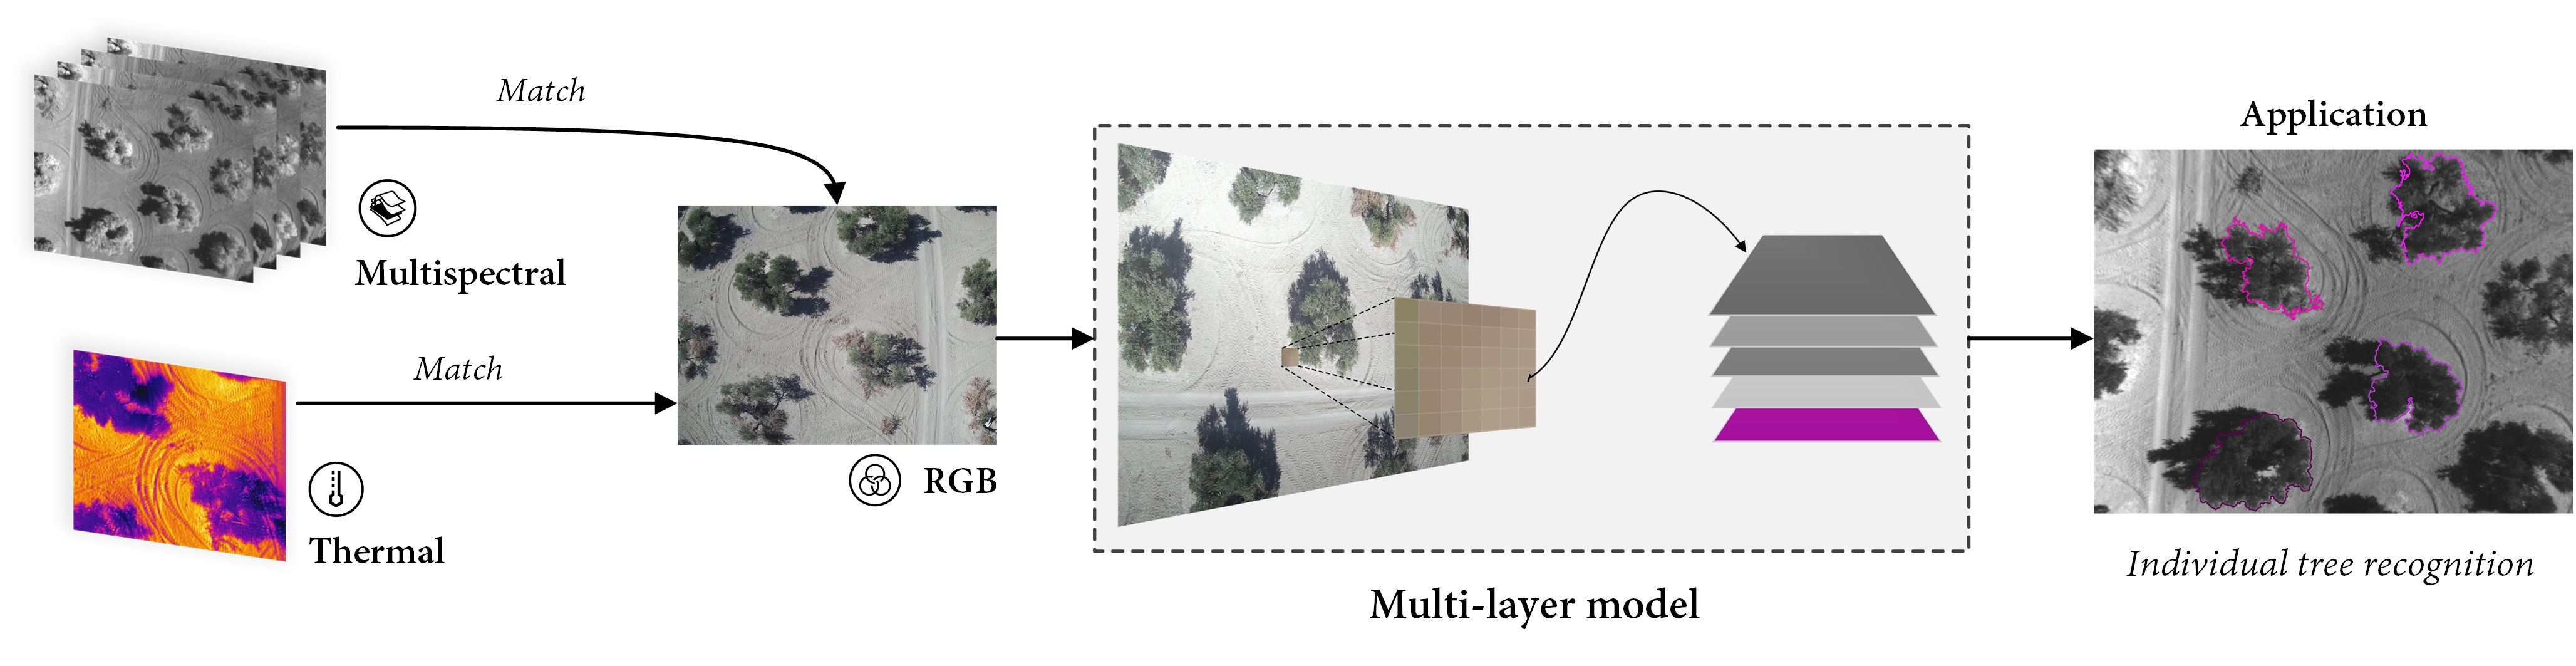
\includegraphics[width=\linewidth]{figs/image_fusion/summary_image_fusion.png}\hspace*{\fill}
    \caption{The fusion of multispectral, thermographic and RGB imagery compose a multi-layer model which is later applied to the characterization of individual trees.}
	\label{fig:image_fusion_framework}
\end{figure*}

The Parrot Sequoia multispectral sensor captures four spectral bands: Green (GRE), Red (RED), Red Edge (\acrshort{reg}) and Near Infrared (\acrshort{nir}). These are acquired by the same device but with different lenses aimed at perceiving different spectral wavelengths. It can be checked that there exists a lack of alignment between them if they are overlapped as collected, as shown in Figure \ref{fig:multispectral_ghost_effect}. At least the following differences were identified: 
\begin{itemize}
    \item Images are translated as a result of each lens working in a \textbf{different fixed position within the multispectral device}. 
    \item \textbf{Every lens has its own optical axis and principal point}. The ideal configuration consists of parallel optical axes that help to solve the misalignment with a simple translation. Even if this was the configuration after manufacturing, the lens calibration deteriorates over time. Indeed, the image metadata shows the viewing conditions of each band with respect to the master one, Green, in what is known as a camera ring. It is defined as a set of cameras which are connected and defined by geometric constraints. Every band defines its own yaw, roll and pitch angles with respect to the master, and thus optical axes cannot be assumed to be parallel.
    \item \textbf{Timestamps are different even for multispectral images triggered at the same time}. It is in the order of \si{\milli\second}, and yet it implies a harder matching because of the \acrshort{uas}'s movement.
\end{itemize}

\begin{marginfigure}[.2cm]
  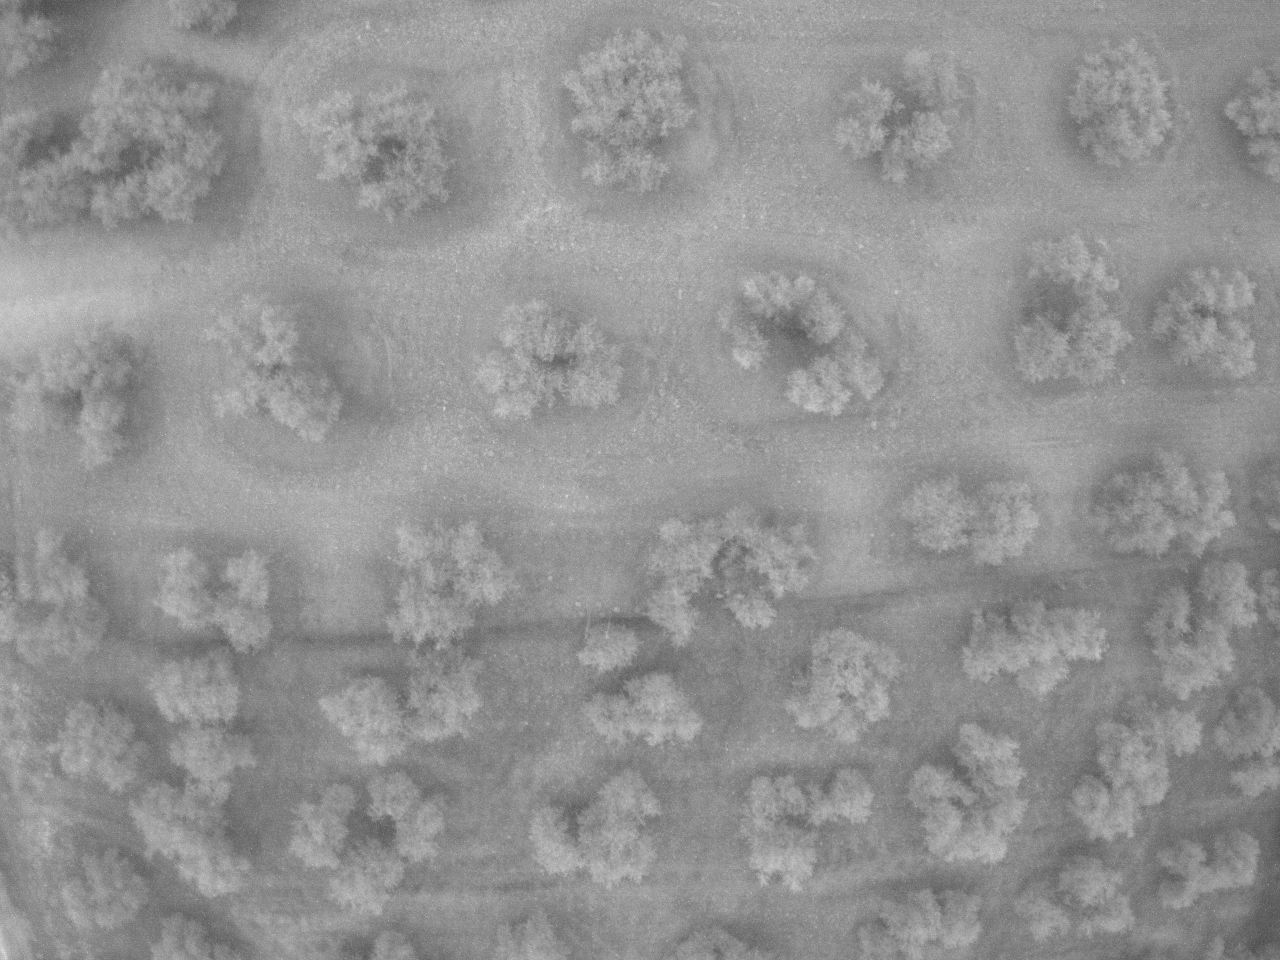
\includegraphics{figs/image_fusion/multispectral_ghost_effect.png}
  \caption{Image ghosting effect obtained by overlapping multispectral bands using $\alpha < 1$.}
  \label{fig:multispectral_ghost_effect}
\end{marginfigure}
The image matching of multispectral data can be achieved with the parameters of the image's metadata, thus relying on sensor calibration. However, another approach is to match images using only colourimetric information. Traditional image-matching approaches, such as \acrshort{sift}, \acrshort{surf} and \acrshort{orb}, do not work well over images from different wavelength intervals that depict surfaces with different radiation in distinct bands. Although there exist variants from \acrshort{sift} that work under photometric differences \cite{park_pi-sift_2008}, these are not as robust as the \textbf{Enhanced Correlation Coefficient (\acrshort{ecc})} \cite{evangelidis_parametric_2008}. Given two images of the same dimensionality, \acrshort{ecc} seeks the matrix that maximizes the intensity correlation of both images, and it is more convenient for our work for the following explained reasons. First, it works by estimating a transformation matrix with variable complexity (see Figure \ref{fig:ecc_motion_models}), ranging from a simple translation ($2 \times 3$) to a homography ($3 \times 4$); the larger the matrix, the more time-consuming the process. Therefore, the motion model can be determined considering the desired time efficiency and what kind of transformations the misalignment presents. Even for the homography, the algorithm has linear complexity ($\mathcal{O}(n)$). The configurable parameters are the number of maximum iterations upon convergence ($n$) as well as the aimed precision ($p$). Another intrinsic parameter is the dimensionality of input images, as lower dimensionality considerably reduces latency.

\begin{marginfigure}[-2cm]
    \centering
    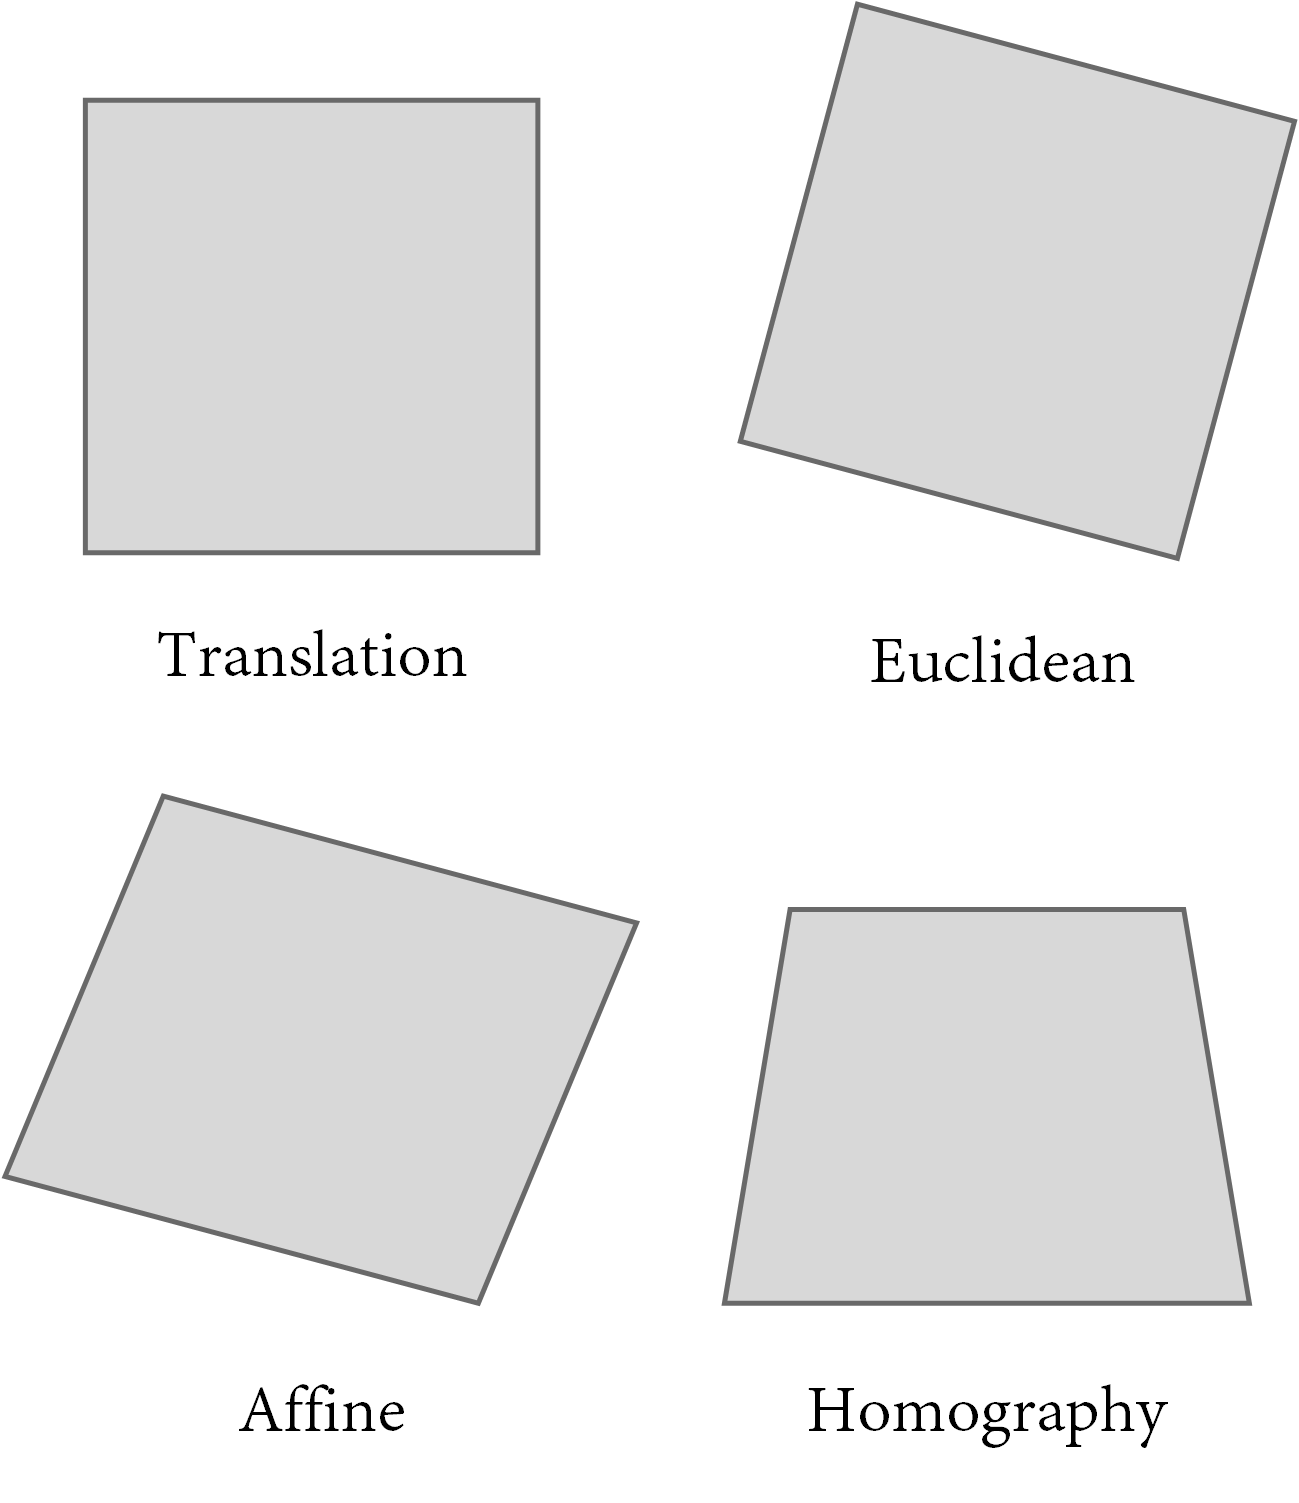
\includegraphics{figs/image_fusion/motion_models.png}
    \caption{Transformation models that can be estimated using \acrshort{ecc}.}
    \label{fig:ecc_motion_models}
\end{marginfigure}

\begin{figure}[ht]
    \centering
    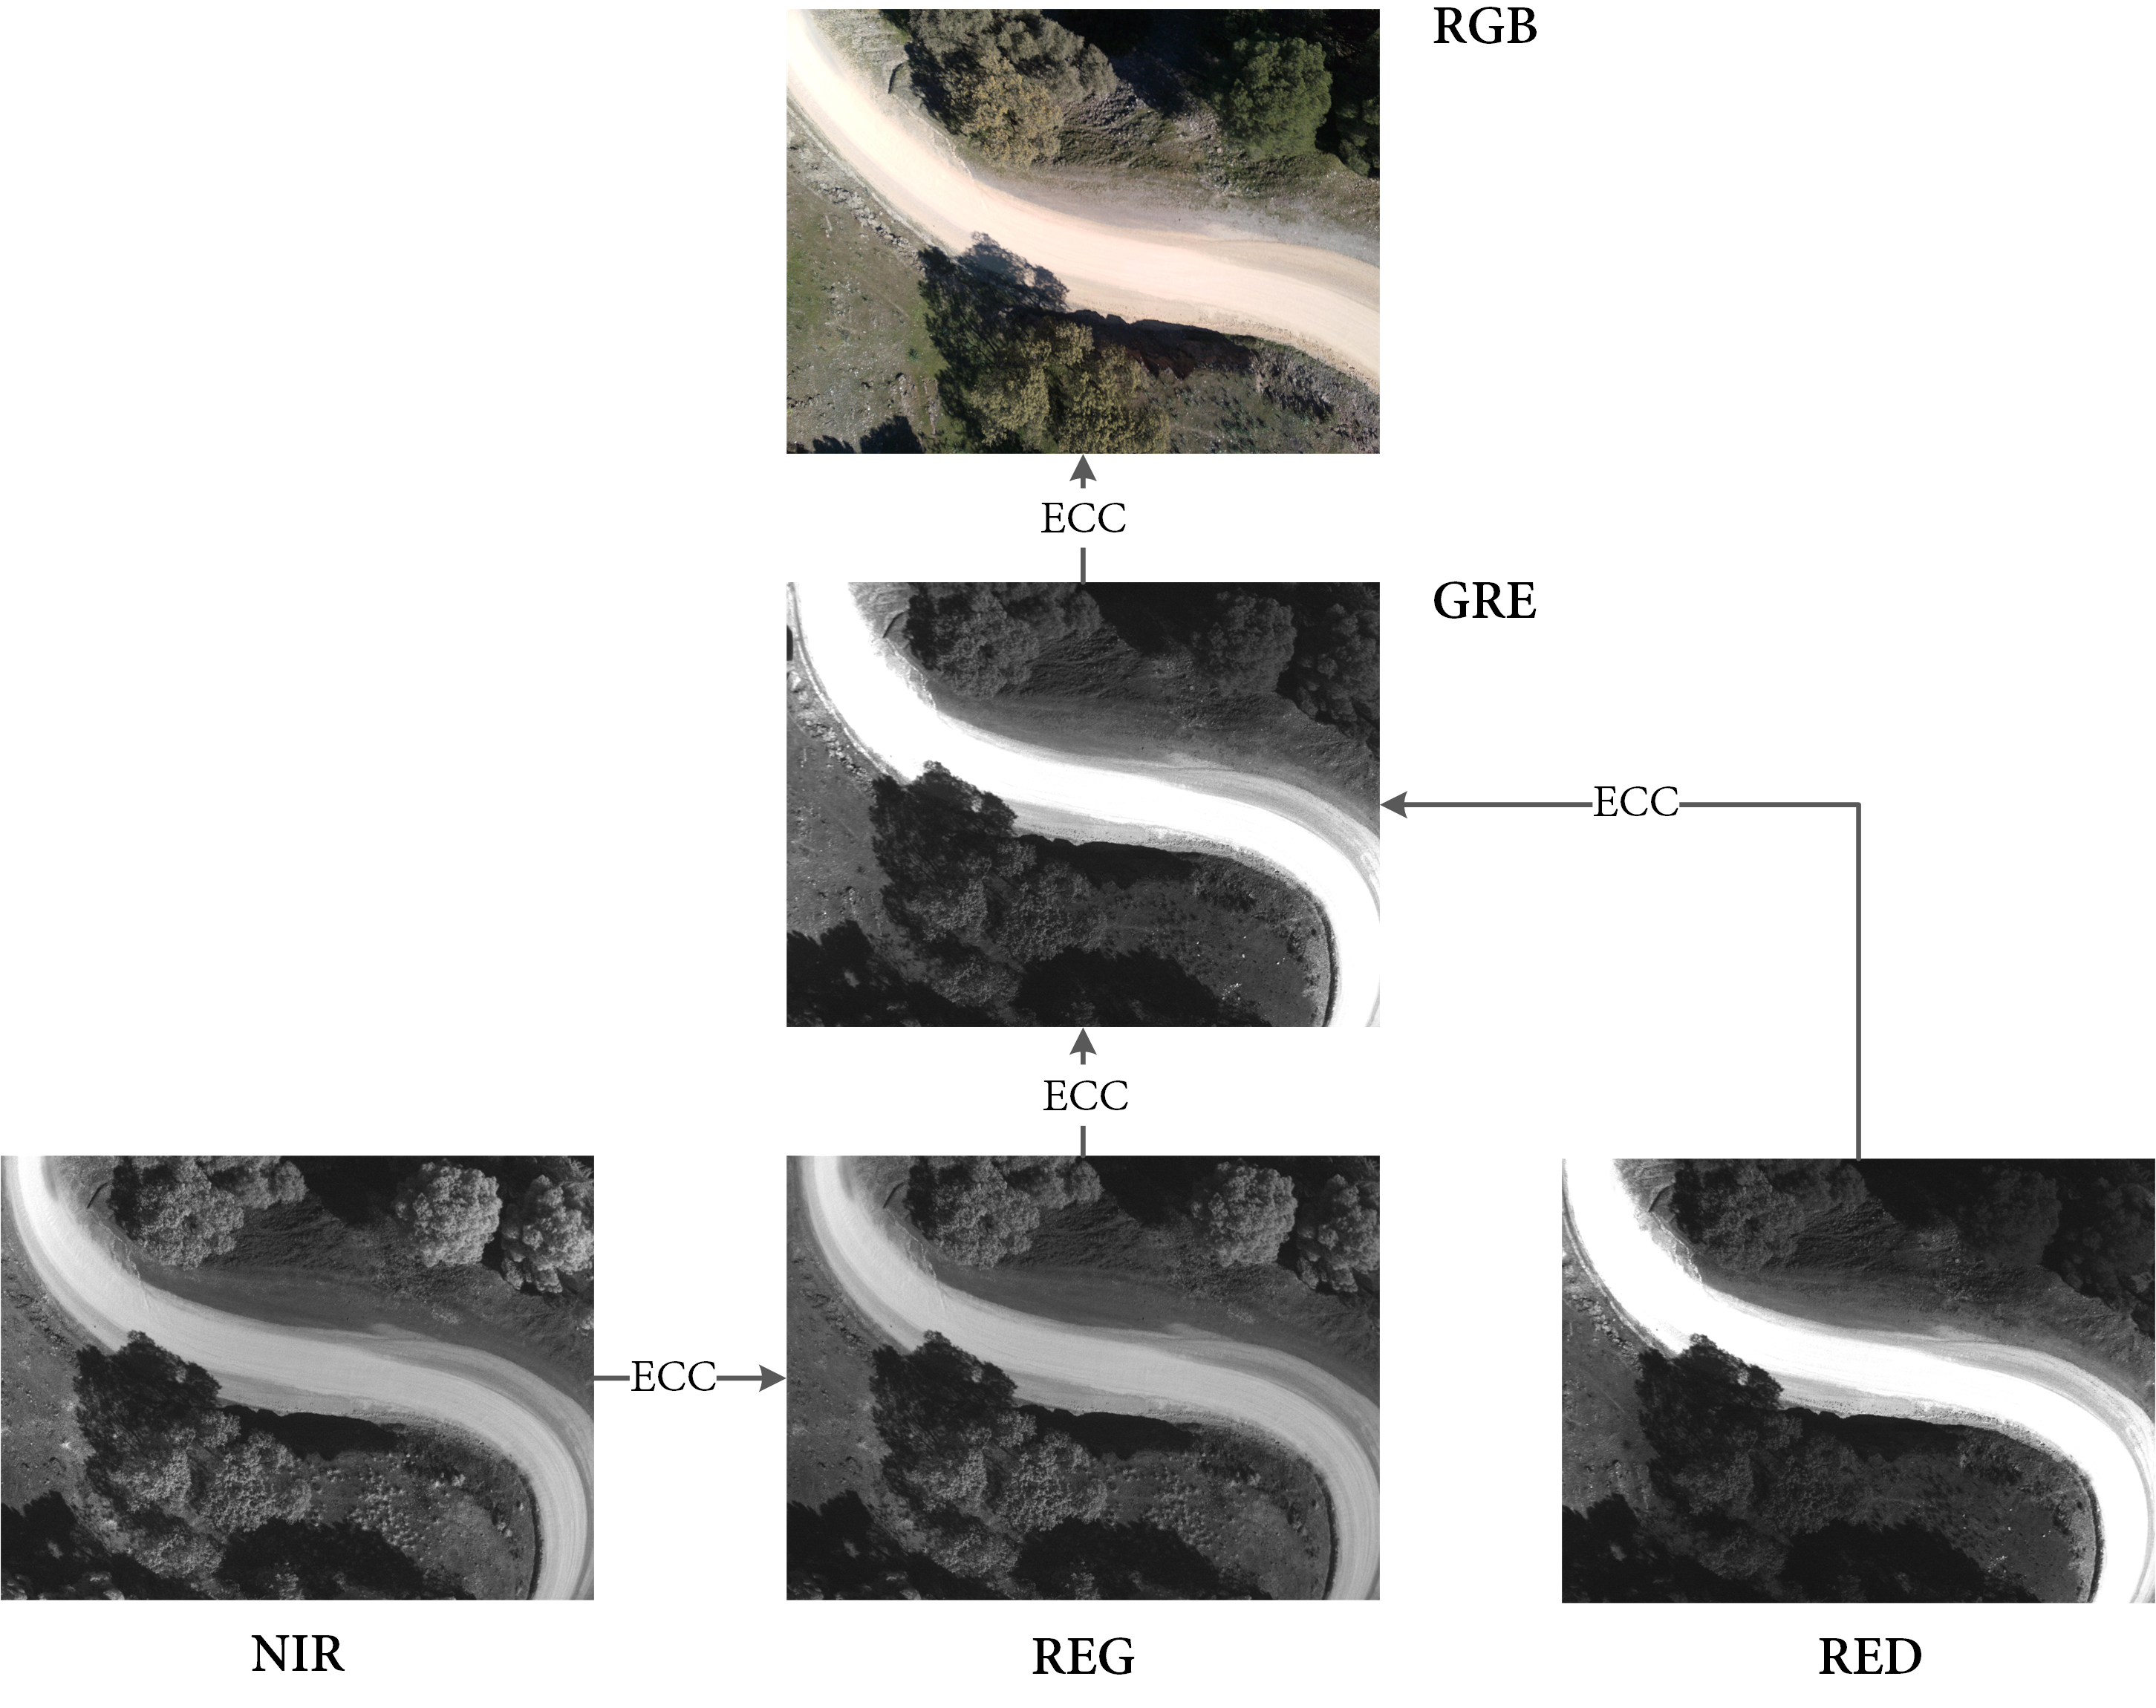
\includegraphics[width=\linewidth]{figs/image_fusion/ecc_hierarchy.png}
    \caption{Hierarchical registration of multispectral imagery.}
	\label{fig:ecc_hierarchy}
\end{figure}

Homography matrices are able to describe any kind of differences among images, but the Euclidean model was observed to be enough for matching multispectral bands. Hence, the complexity was reduced by estimating a matrix of size $2 \times 3$ explaining translation, rotation and scaling, with the first being the most relevant. The procedure can be further improved by first matching those images which are more similar in terms of intensity. According to the peculiarities of multispectral images, these are fused hierarchically rather than sequentially. With this approach, images with more similar intensity are first registered. More specifically, the pipeline depicted in Figure \ref{fig:ecc_hierarchy} is followed: $\textit{GRE} \rightarrow \textit{RGB}$, $\textit{RED} \rightarrow \textit{GRE} \rightarrow \textit{RGB}$, $\textit{REG} \rightarrow \textit{GRE} \rightarrow \textit{RGB}$ and $\textit{NIR} \rightarrow \textit{REG} \rightarrow \textit{GRE} \rightarrow \textit{RGB}$. Still, each image is only registered once, as the whole chain concatenation is computed using matrix composition. However, the algorithm does not always converge to the expected precision for every pair of images nor the results are optimal. When this occurs, the resulting quadrilateral shape is very distorted, and it can be identified by setting a threshold angle, $\beta$, that is compared against the angles enclosed in the obtained shape. Additionally, the transformed result can have areas null values, as occurred with the correction of fisheye distortion. Once again, the minimum area to be cropped can be calculated as defined in Equation \ref{eq:matrix_corners}. It cannot be simply computed from the lower left and upper right corners, $[0, 0]$ and $[w - 1, h - 1]$, since Euclidean transformations also involve rotations. Thus, it is not enough to check two non-adjacent corners.

The hierarchical alignment of multispectral images is constructed on the basis of the similarity between multispectral bands, as shown in Figure \ref{fig:multi_band_correlation}. It shows the similarity between any pair of bands by calculating the normalized correlation coefficient (\acrshort{cc}), which shows how similar two grayscale images are. For the sake of simplicity, the Green image is considered the root as in the camera ring. Accordingly, Figure \ref{fig:multi_band_correlation} justifies the hierarchy shown in Figure \ref{fig:ecc_hierarchy}. Note that \acrshort{nir} and \acrshort{reg} layers are reciprocally the most similar. However, \acrshort{reg} images are more similar to the root, Green, and thus \acrshort{nir} layers were aligned to \acrfull{reg} images.

\begin{figure*}
    \centering
    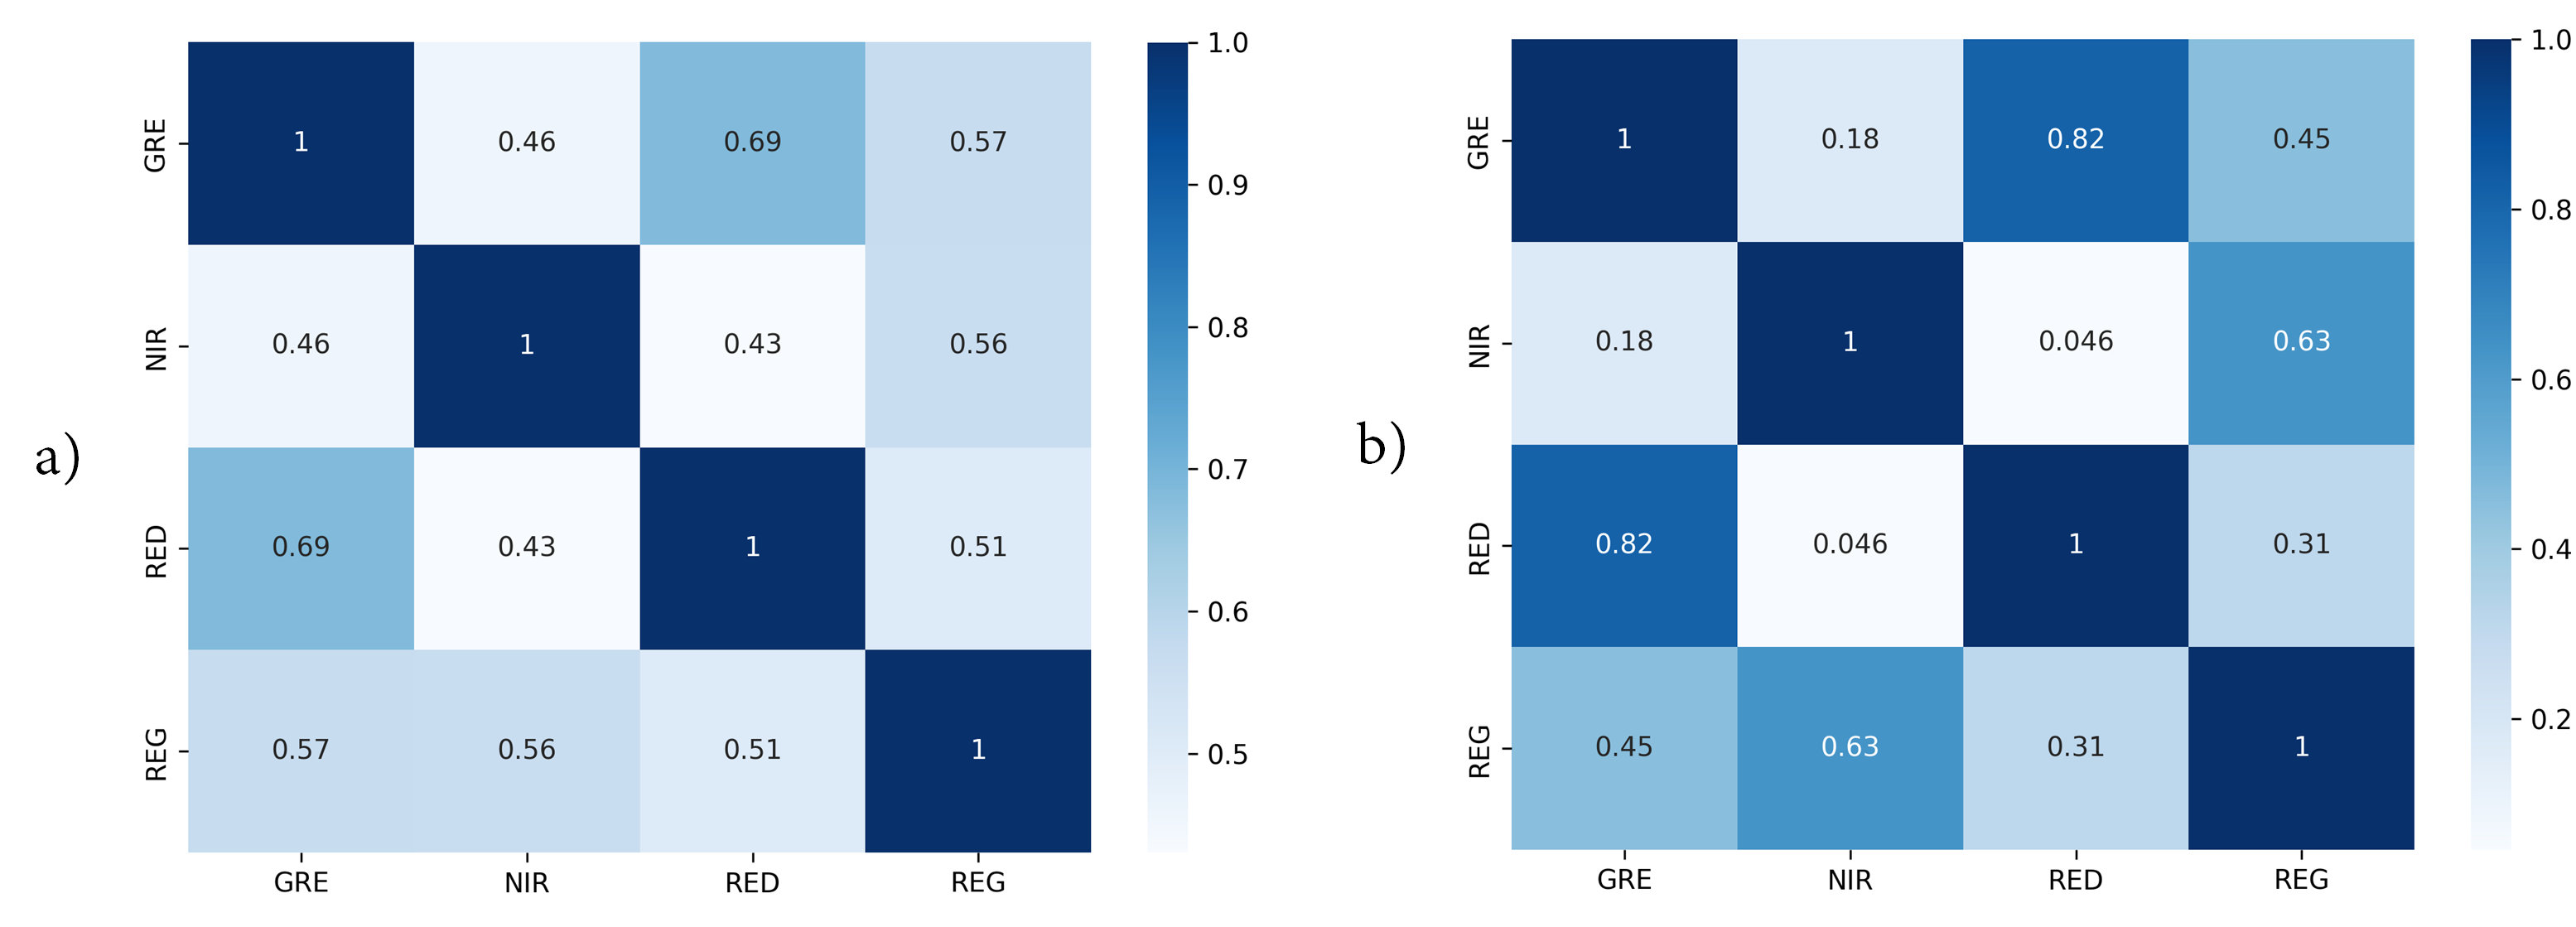
\includegraphics{figs/image_fusion/confusion_matrices.png}
    \caption{Confusion matrices depicting the similarity of multispectral images in three different datasets.}
    \label{fig:multi_band_correlation}
\end{figure*}

\section{Matching RGB and multispectral imagery}

\begin{figure*}
    \centering
    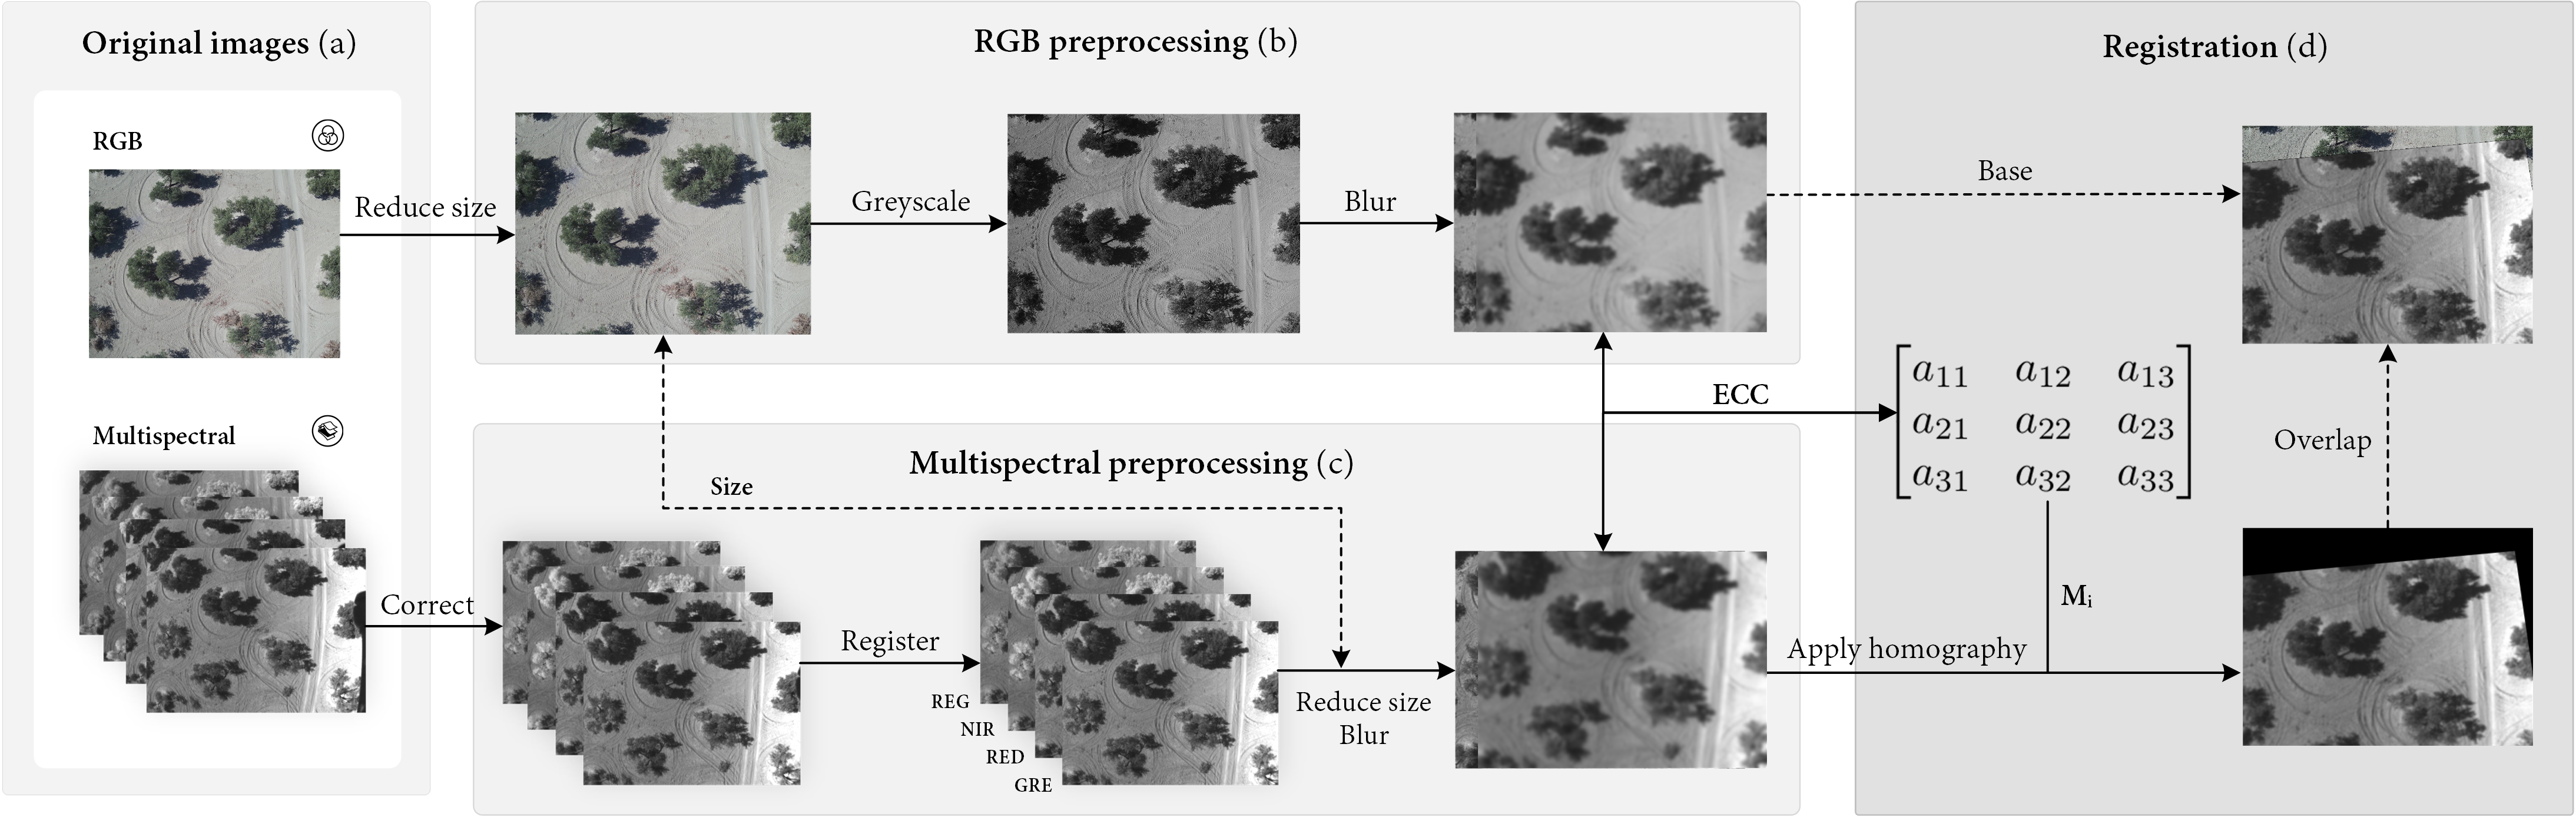
\includegraphics{figs/image_fusion/multispectral_rgb_registration.png}
    \caption{Image-matching of \acrshort{rgb} and multispectral datasets. The blur size was increased for a better understanding of the figure.}
    \label{fig:rgb_multi_registration}
\end{figure*}

The contribution of \acrshort{rgb} imagery to this model is to add more accurate geopositioning data. However, multispectral and \acrshort{rgb} datasets were not acquired by the same device in this study, nor they were synchronized on the triggering. Thus, images to be matched are selected according to the timestamp, and yet, the differences can be in the order of seconds. Similarly to the previous case study, the \acrshort{ecc} algorithm suits well the matching of \acrshort{rgb} and multispectral imagery since they have some relevant differences concerning the observed intensity. Instead of matching every multispectral image, only the Green band is required according to the hierarchy proposed in Figure \ref{fig:ecc_hierarchy}.

\acrshort{rgb} images have higher dimensionality than multispectral images, and therefore, the former was downscaled to match the size of the latter. The \acrshort{ecc} algorithm can be applied at a sub-pixel level and its parameters can be configured for a fine-grained registration. Furthermore, a faster convergence can be achieved by blurring both images, despite including the overhead from blurring. The complete workflow is shown in Figure \ref{fig:thermal_registration}, using a blur mask of size 3, a high number of iterations, $n \gets 400$, and a high precision factor, $p \gets 1^{-60}$. The values of these parameters are further discussed in Section \ref{sec:image_fusion_evaluation}, whereas Figure \ref{fig:rgb_multi_registration_result} shows an example of this matching procedure.

\begin{figure}[ht]
    \centering
    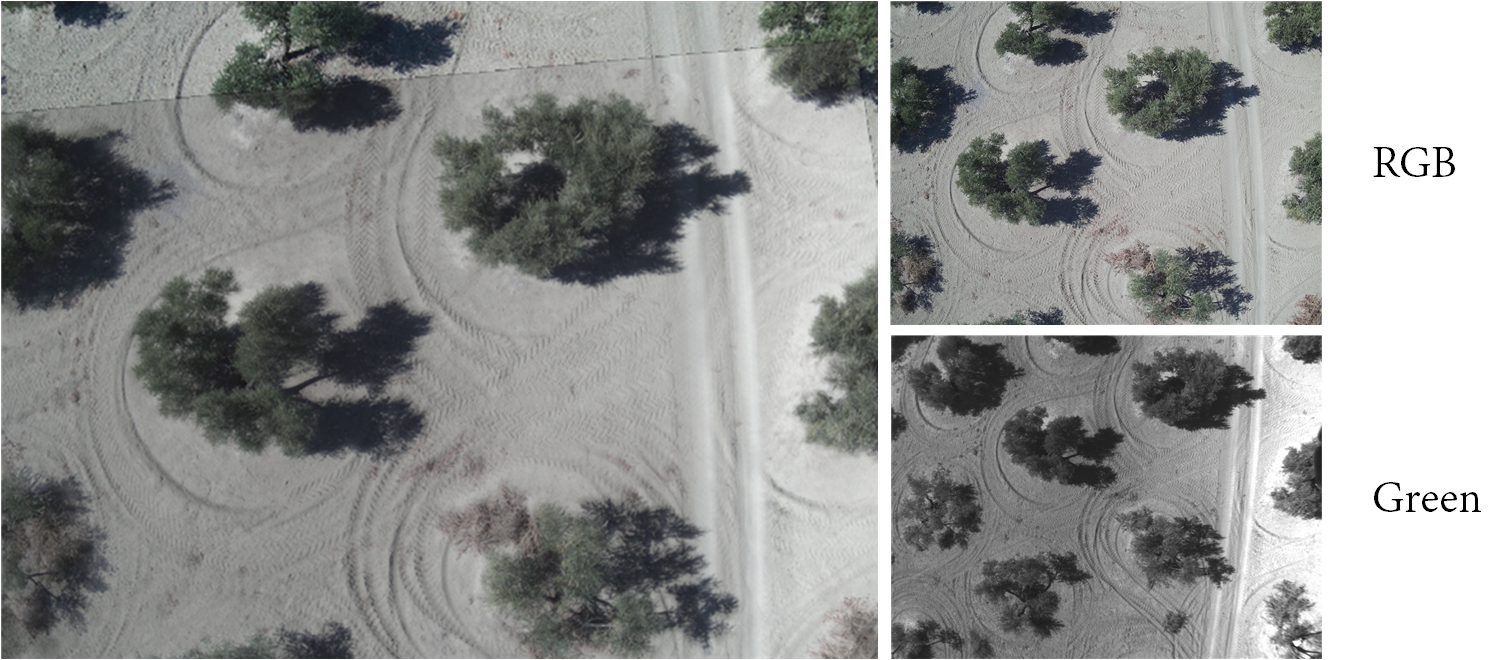
\includegraphics{figs/image_fusion/rgb_multispectral_registration_result.png}
    \caption{An example of image-matching between an \acrshort{rgb} image and the Green multispectral band, with the initial images being depicted on the right side.}
    \label{fig:rgb_multi_registration_result}
\end{figure}

\section{Matching RGB and thermographic images}

\begin{figure*}
    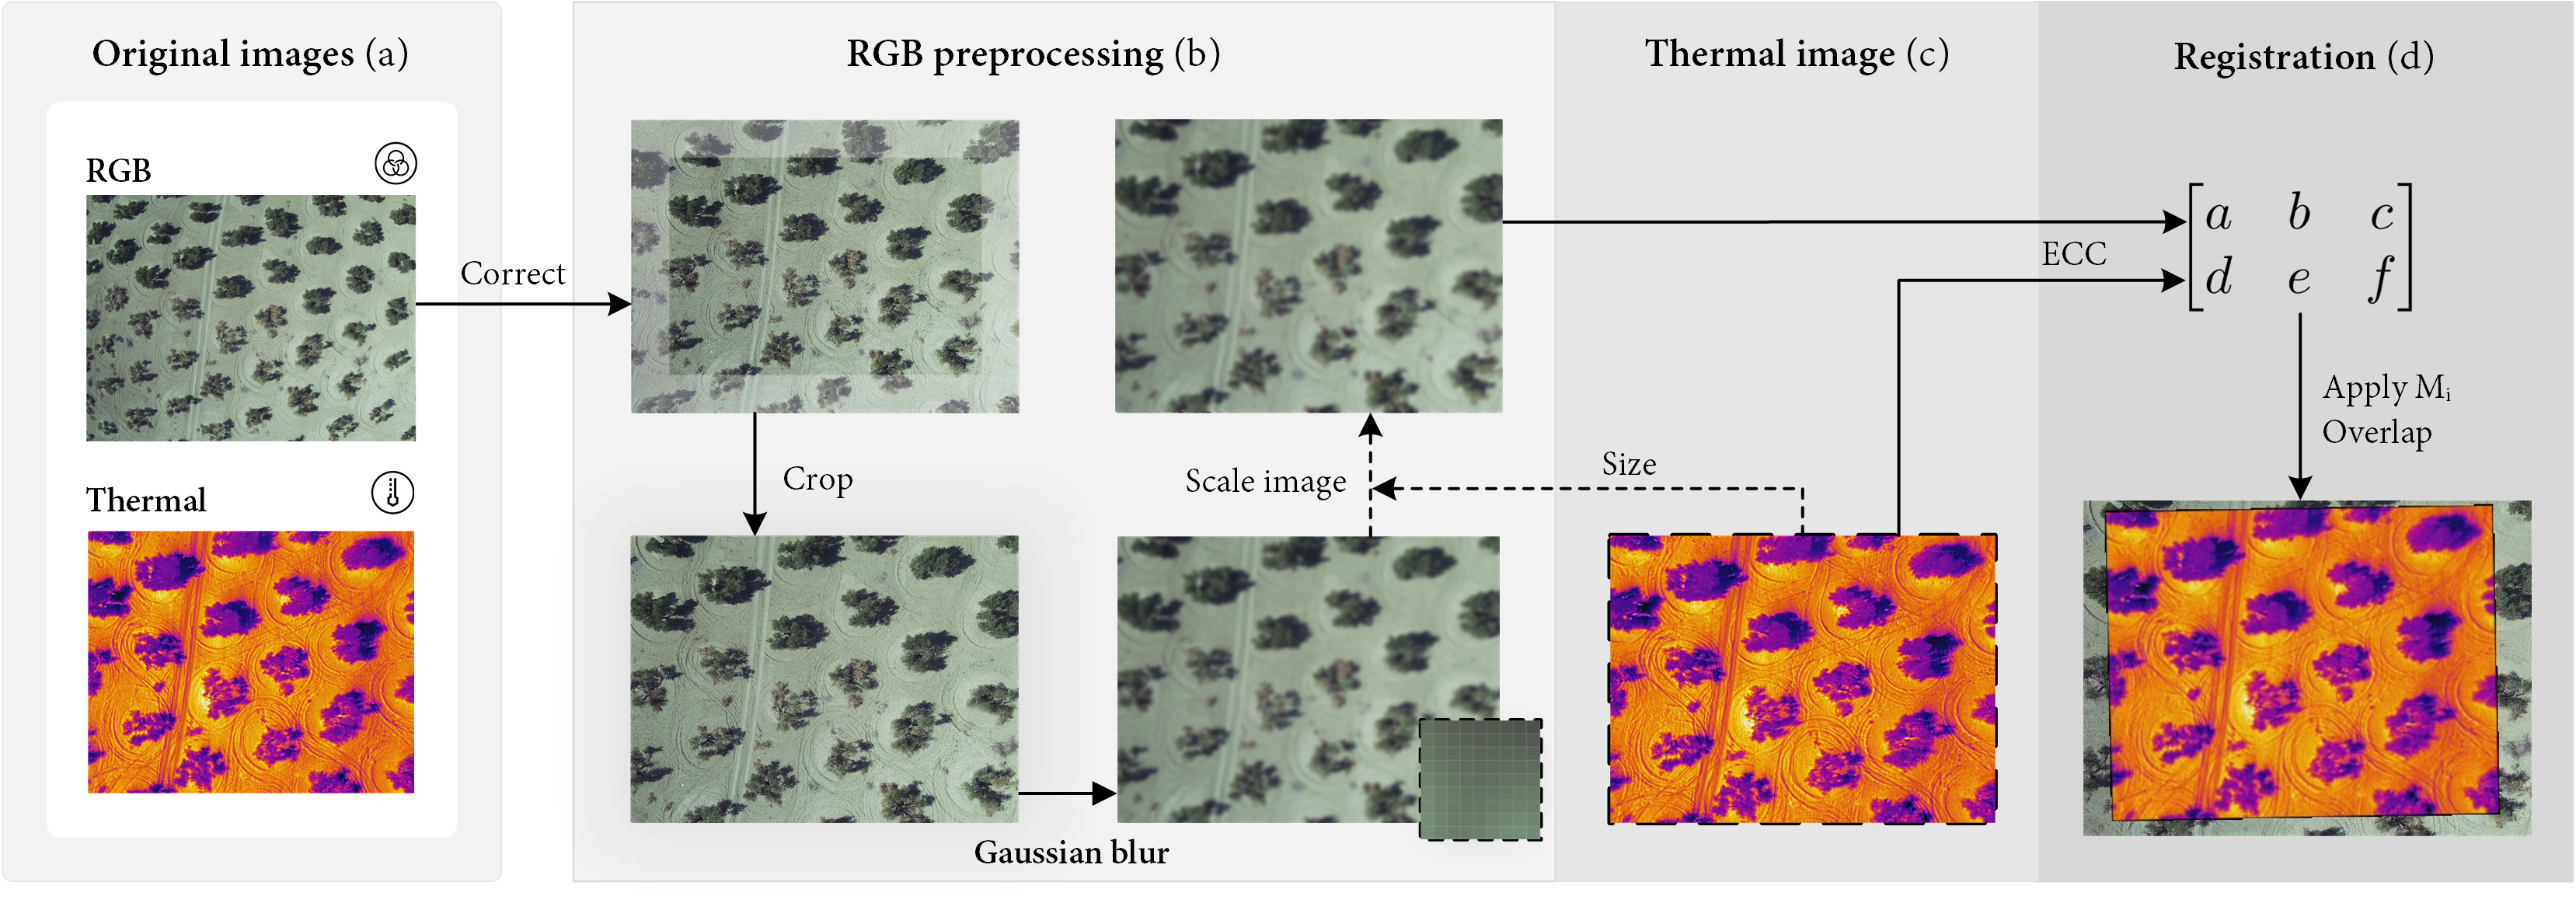
\includegraphics{figs/image_fusion/thermal_registration.png}
    \caption{Flow chart of the image-matching procedure between \acrshort{rgb} and infrared imagery.}
    \label{fig:thermal_registration}
\end{figure*}

The last step of this multi-layer system is to match thermal and \acrshort{rgb} imagery, with \acrshort{rgb} images being the link between multispectral and thermal datasets. Previous shortcomings related to different triggering timestamps are here alleviated since both kinds of images are captured by the same device. Still, there exist large differences in the optical acquisition of \acrshort{rgb} and thermal images. The \acrshort{rgb} lens captures a wider area with a fisheye distortion model, whereas the thermal lens has a more narrowed field of view. Similarly to multispectral images, the dissimilarities between these two types of images can be attributed to translations resulting from variations in the physical distance between lenses, as well as rotations that arise from the deployment of distinct optical systems. The latter factor is particularly significant, as it poses a challenge for accurately extracting the region of interest captured by both devices.

\begin{marginfigure}[-2cm]
    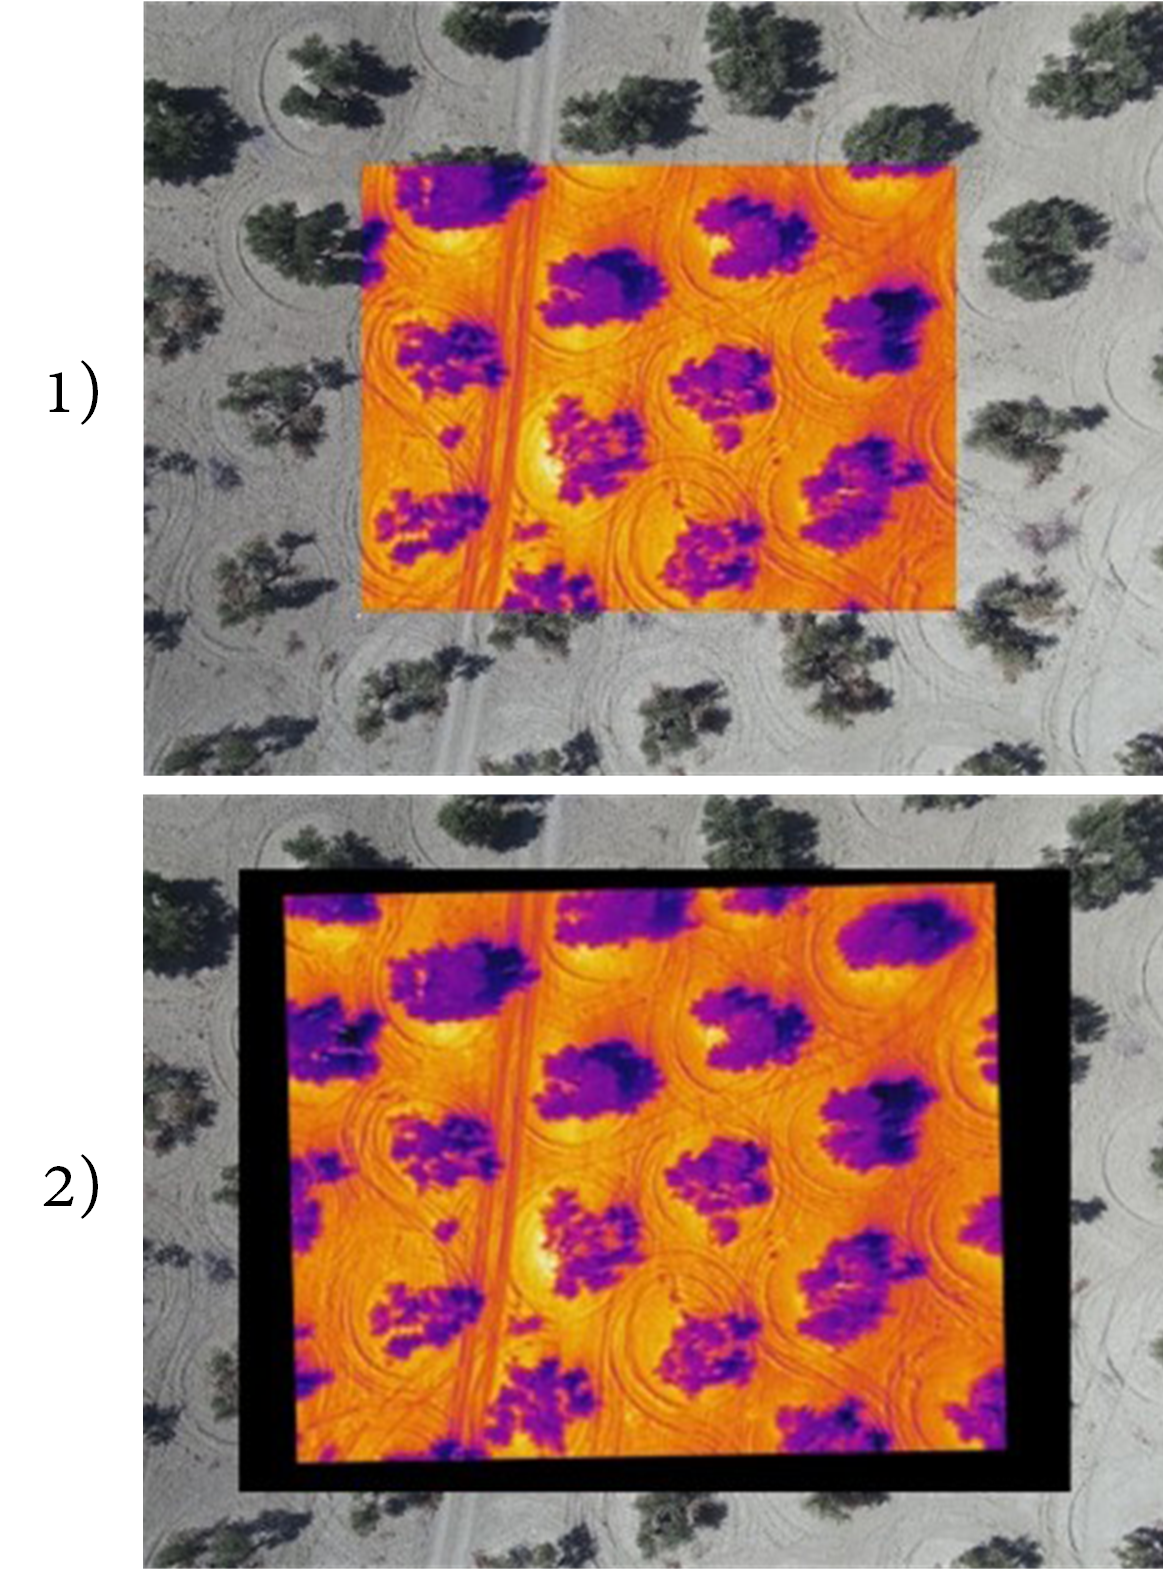
\includegraphics{figs/image_fusion/thermal_comparative.png}
    \caption{Matching of \acrshort{rgb} and thermal images using 1) an \acrshort{rgb} area smaller than thermal images and 2) a larger \acrshort{rgb} area. }
    \label{fig:thermal_comparative}
\end{marginfigure}
After identifying the shortcomings, it was observed that an affine transformation sufficed for addressing them. Translation and rotation were found to be effective in mitigating the visual disparities between the \acrshort{rgb} and thermal imagery, while scaling was necessary to ensure appropriate alignment between the two images. Two approaches could be employed to achieve a successful match: a) selecting a larger area of the \acrshort{rgb} image that fully encompasses the thermal image, resulting in some null values, or b) selecting a smaller area that does not cover the entire thermal image, thus addressing the previously mentioned issue (see Figure \ref{fig:thermal_comparative}). To improve the response time, the \acrshort{rgb} images were downscaled to fit the thermal dimensions. The precision factor and the number of iterations were fine-tuned to achieve accurate registration. The complete procedure is outlined in Figure \ref{fig:thermal_registration}.

\section{Segmentation of individual trees}

The proposed framework enables obtaining \acrshort{rgb}, multispectral and thermographic data from an area of interest. This stack of layers can be further applied to the temporal tracking of individual trees. More specifically, multispectral images are sensitive to vegetation and thus can help in the identification of trees. Once identified, points belonging to each one can be further analyzed to extract vegetation indices such as \acrshort{ndvi}. 

The observed surface reflectance, $f(\theta)$, exhibits distinctive peaks where the reflectance of vegetation reaches a maximum value. This contrast between layers with higher and lower reflectance enables differentiation between soil and canopy. While the data lacks the finer resolution of hyperspectral data, the relative maximum and minimum reflectance values for vegetation are visible in the \acrshort{nir} and Red layers, respectively. As soil reflectance is generally constant or low across these layers, it can be effectively filtered out. Consequently, applying the formula $\textit{\acrshort{nir}} - \textit{Red}$ yields the outcome depicted in Figure \ref{fig:contour_extraction}.

The following steps are performed before the image subtraction:
\begin{enumerate}
    \item \textbf{Gaussian blur} to smooth the image colour and remove noise.
    \item \textbf{Image thresholding} to isolate the vegetation areas.
    \item \textbf{Extraction of the hierarchy of contours}. Contours that are inside another one, those that belong to small low vegetation or noise, and partially visible (cropped) contours are all deemed irrelevant. It is easy to identify the latter issue as cropped contours have horizontal or vertical edges in the image boundaries.
\end{enumerate}

\begin{figure*}[hbt]
	\centering
	\includegraphics{figs/image_fusion/contour_retrieval.png}
	\caption{Transformation of multispectral images to distinguish vegetation and soil.}
	\label{fig:contour_extraction}
\end{figure*}

\begin{figure}[hbp]
    \centering
    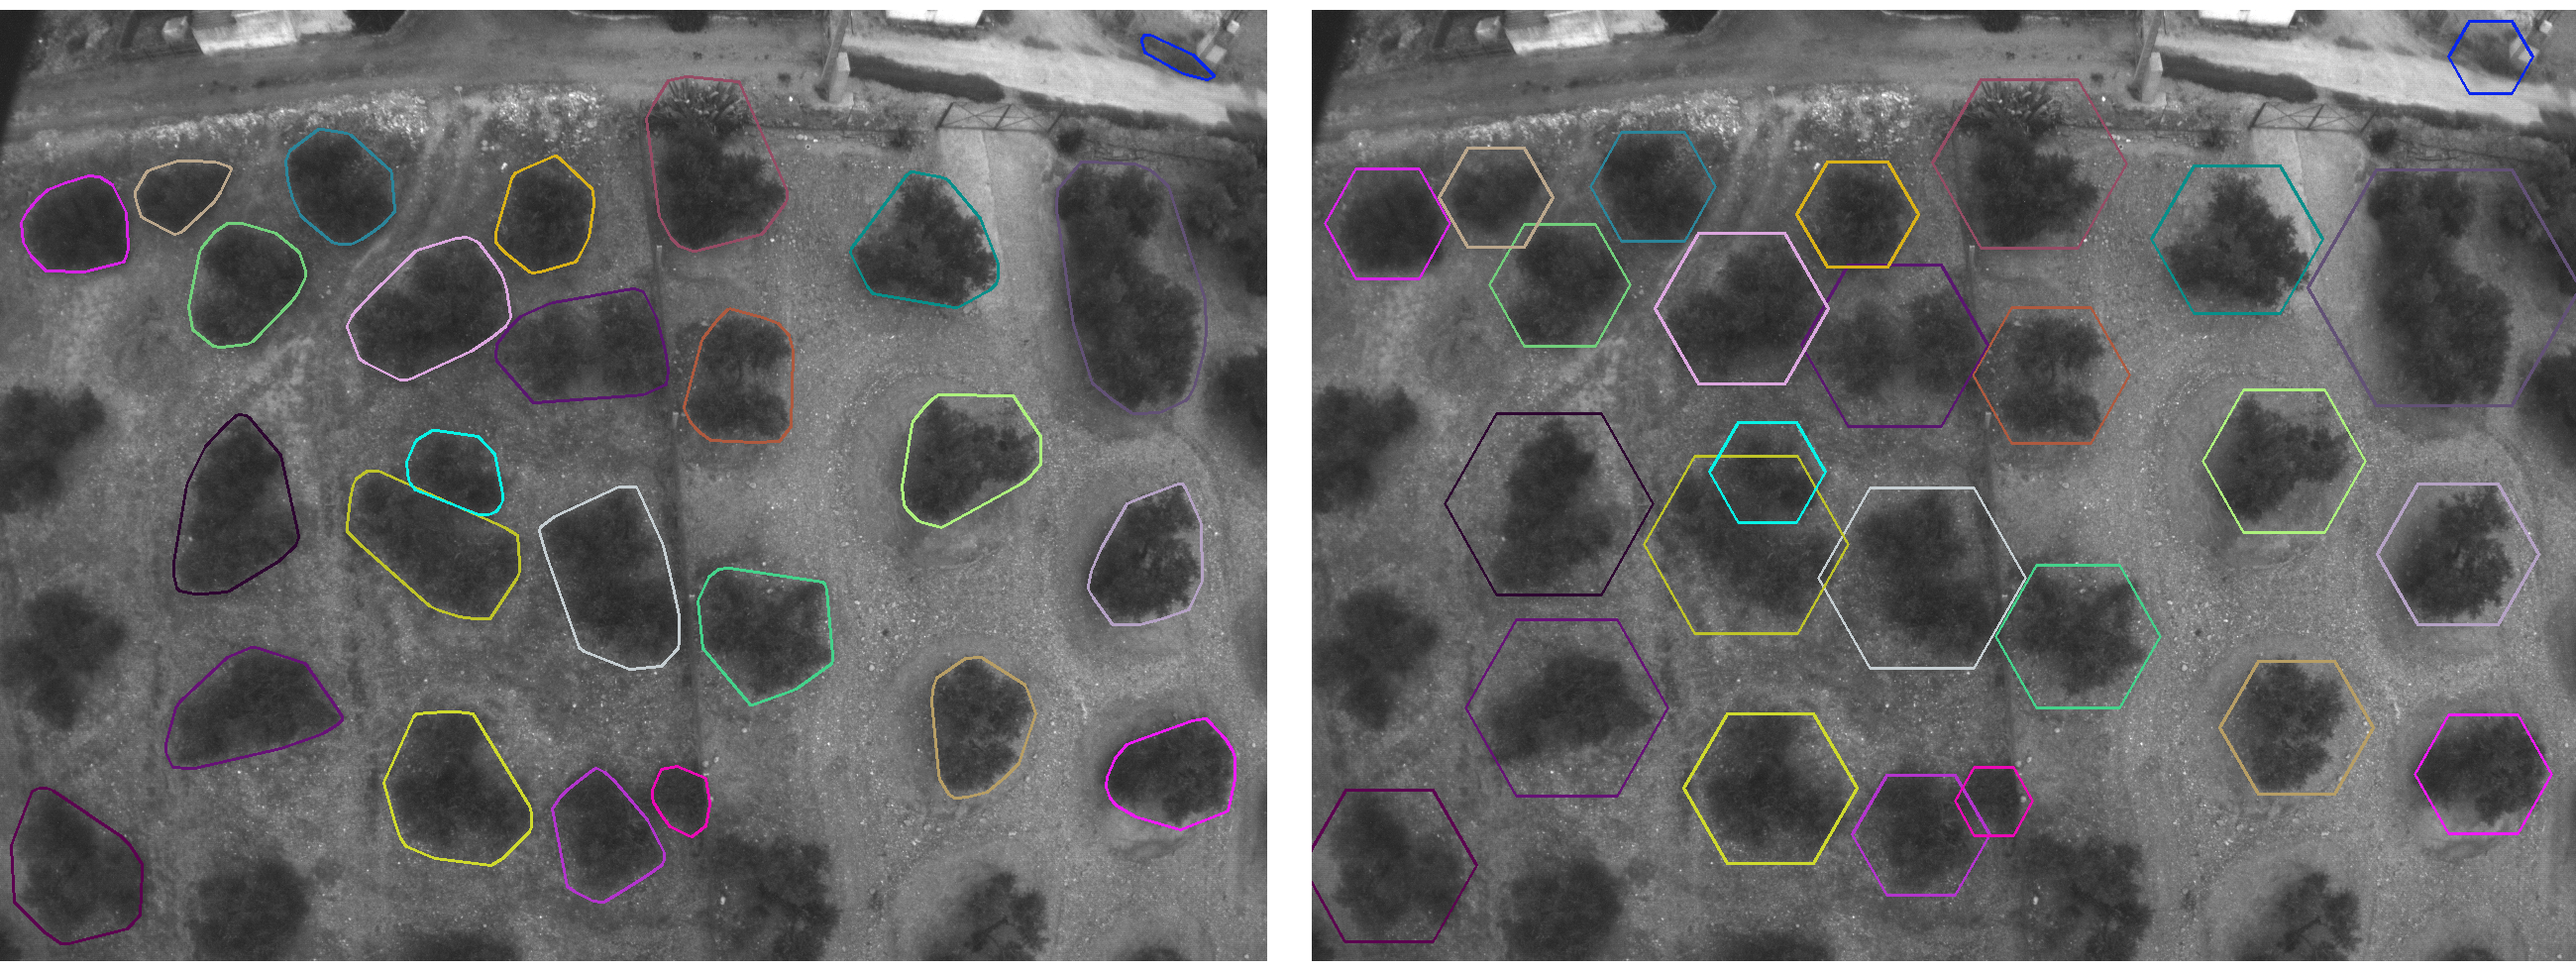
\includegraphics[width=1\linewidth]{figs/image_fusion/convex_hull_contours.png}
    \caption{Conversion of polygons into convex and hexagonal hulls.}
    \label{fig:convex_hull_contours}
\end{figure}

The identification of individual trees is determined by the size of a blur mask, the maximum area to be discarded, and a threshold value. This threshold must be large enough to prevent the merging of closely located trees. Although this procedure produces shapes with a high \acrshort{lod}, they typically contain hundreds of points that can be simplified using a convex hull \cite{sklansky_finding_1982} or other polygons, such as hexagons (see Figure \ref{fig:convex_hull_contours}).

\section{Results and discussion}
\label{sec:image_fusion_evaluation}

This methodology has been evaluated with four different datasets depicting olive orchards located in Jaén, a Southern region of Spain. The first three datasets have multispectral and \acrshort{rgb} images, whereas the last one comprises \acrshort{rgb} and thermal imagery. The main study area covers two hectares of olive trees in which the proposed methodology has been checked. Figure \ref{fig:image_fusion_study_area} presents a general overview of the main study area.

\begin{figure*}[htb]
    \centering
    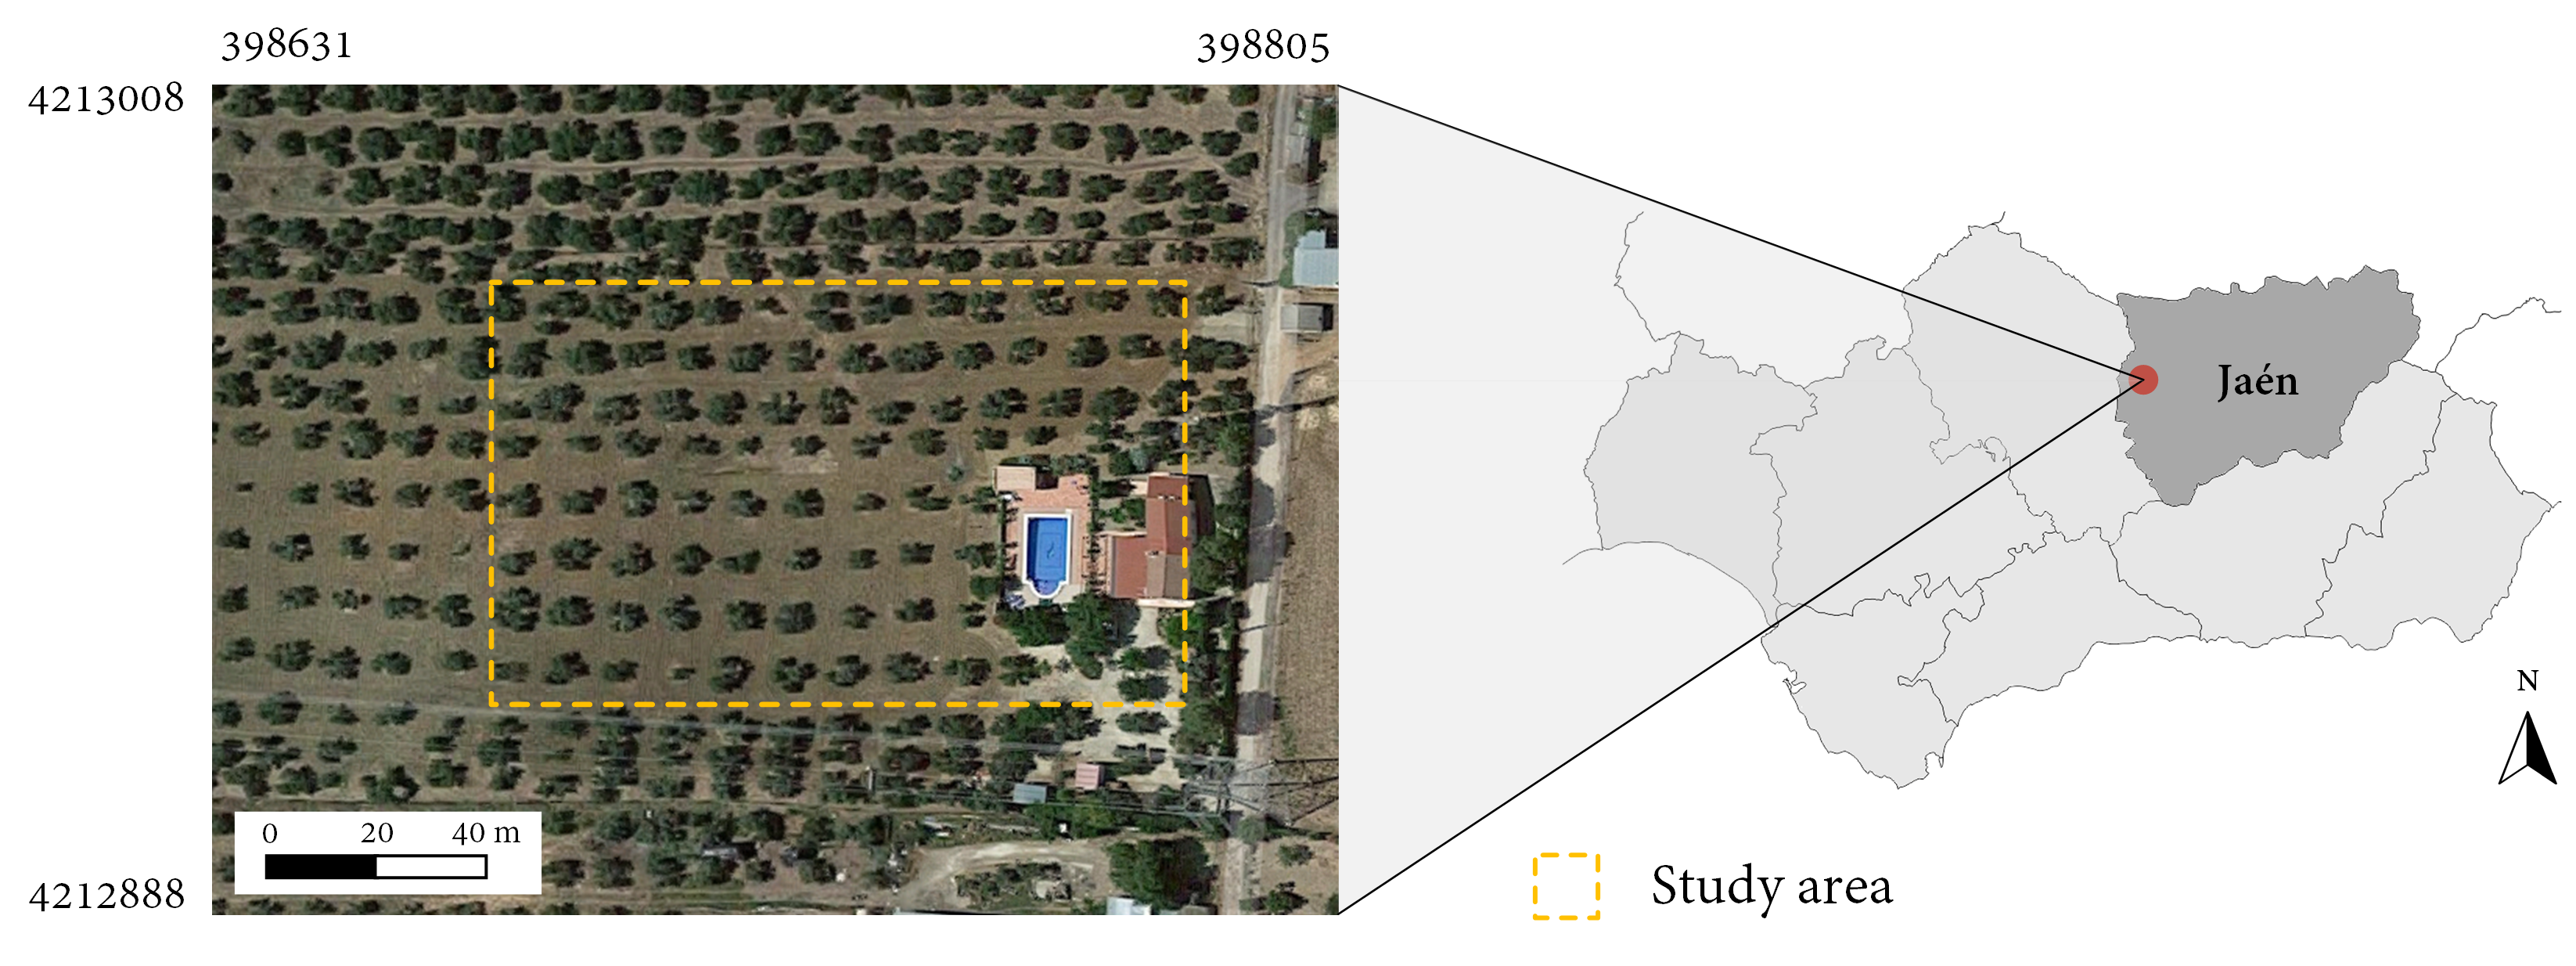
\includegraphics[width=\linewidth]{figs/image_fusion/study_area.png}
    \caption{An overview of the study area presented in the Universal Transverse Mercator (\acrshort{utm}) coordinate system.}
    \label{fig:image_fusion_study_area}
\end{figure*}

The measurements were carried out on a computer equipped with an Intel Core i7.6700 processor running at 3.4GHz, 16GB RAM, an NVIDIA GTX 1070 graphics card with 8GB RAM, and Windows 10 operating system (\acrshort{os}). The \acrshort{ecc} algorithm was implemented using the Open Source Computer Vision Library (\acrshort{opencv}) in a C++ application. The accuracy of the matching process was assessed using the normalized \acrshort{cc} metric, which was defined as shown in Equation \ref{ec:correlation_coefficient}. The \acrshort{cc} metric produces a coefficient $\rho \in [0, 1]$ that measures the similarity between two images - the source and the template. Although it is not a perfect measure of the similarity between images, it estimates the intensity difference between two images and is useful for evaluating the matching accuracy. Finally, the images to be compared were randomly selected from the four datasets.
\begin{equation}
    \label{ec:correlation_coefficient}
    \textit{CC} = \frac{\sum_{x=1}^{w} \sum_{y=1}^{h} T_{x,y} \cdot I_{x,y}}{\sqrt{\sum_{x=1}^{w} \sum_{y=1}^{h} T_{x,y}^{2} \cdot \sum_{x=1}^{w} \sum_{y=1}^{h} I_{x,y}^{2}}}
\end{equation}
with $w$ and $h$ being the width and height of both $T$ and $I$ images.

The response time and obtained accuracy were checked against several configurations with the following parameters: 
\begin{itemize}
    \item \textbf{Precision to converge}. The closer it gets to zero, the harder is for the algorithm to converge.
    \item \textbf{Number of iterations}. A larger number of iterations helps to give some room for the algorithm to converge. 
    \item \textbf{Image size}. A smaller dimensionality helps to decrease the response time and achieve faster convergence, and it does not necessarily lead to worse matching results. 
\end{itemize}

\subsection{Multispectral registration}

To evaluate the accuracy of the proposed image-matching methodology, four experiments were conducted using the four multispectral bands. The initial normalized \acrshort{cc} values are presented in Table \ref{table:multispectral_base_correlation} to demonstrate the improvement achieved by the four image-matching experiments. Since the dimensionality of the multispectral images was already low, downsampling was unnecessary.

\renewcommand{\arraystretch}{1.05}
\begin{table}[H]
    \caption{Normalized \acrshort{cc} between original multispectral images. }
    \label{table:multispectral_base_correlation}
    \begin{tabular}{l@{\hskip 0.3in}l|c@{\hskip 0.3in}c@{\hskip 0.3in}c}
        \toprule
        & & GRE-RED & GRE-\acrshort{nir} & GRE-\acrshort{reg} \\
        \cmidrule{1-5}
        Dataset & Viewpoint & $\rho$ & $\rho$ & $\rho$ \\
        \cmidrule{1-5}
        \multirow{3}{*}{1} & 1 & 0.8954 & 0.8777 & 0.9306\\
        & 4 & 0.9777 & 0.9381 & 0.9618\\
        & 6 & 0.9756 & 0.9520 & 0.9727\\
        \cmidrule{1-5}
        \multirow{4}{*}{2} & 37 & 0.9286 & 0.9100 & 0.9371\\
        & 48 & 0.9265 & 0.8918 & 0.9316\\
        & 58 & 0.9146 & 0.8878 & 0.9242\\
        & 53 & 0.9777 & 0.9381 & 0.9618\\
        \cmidrule{1-5}
        \multirow{8}{*}{3} & 9 & 0.9669 & 0.9545 & 0.9714\\
        & 35 & 0.9578 & 0.9453 & 0.9739\\
        & 78 & 0.9707 & 0.9504 & 0.9672\\
        & 107 & 0.9602 & 0.9537 & 0.9686\\
        & 136 & 0.9755 & 0.9612 & 0.9692\\
        & 141 & 0.9732 & 0.9551 & 0.9744\\
        & 142 & 0.9728 & 0.9375 & 0.9656\\
        & 144 & 0.9731 & 0.9316 & 0.9622\\
        \cmidrule{1-5}
        \multicolumn{2}{r|}{\textbf{Average}} & \textbf{0.9564} & \textbf{0.9323} & \textbf{0.9581}\\
        \bottomrule
    \end{tabular}
    \normalsize
\end{table}
\renewcommand{\arraystretch}{1}

The first experiment used parameters that were close to the optimal configuration but resulted in a higher response time. The results in Table \ref{table:multispectral_rgb_correlation} indicate that this approach achieved good alignment for most images, but not for those with significant intensity differences among several spectral bands, such as human-made objects. Nonetheless, the images were well-aligned according to visual inspection. The second test aimed to decrease the response time at the expense of a lower \acrshort{cc}. The third experiment used an intermediate configuration that achieved a high \acrshort{cc} while also reducing the latency. Finally, the fourth experiment downscaled the image size by $1/3$, achieving a higher \acrshort{cc} with a lower response time. However, as noted by visual inspection, this approach returned worse results for some images. 

\textit{The four experiments were configured as follows, where $n$ is the number of iterations and $p$ is the aimed precision. Test 1: $n \gets 30, p \gets 1^{-10}$, test 2: $n \gets 15, p \gets 1^{-2}$, test 3: $n \gets 15, p \gets 1^{-10}$ and test 4: $n \gets 150, p \gets 1^{-60}$}.

\renewcommand{\arraystretch}{1.1}
\begin{table*}
    \footnotesize
    \caption{Normalized correlation coefficient and response time on the matching of a random subset of multispectral images over four different tests.}
    \label{table:multispectral_correlation_registration}
    \begin{tabular}{ll|cccr|cccr}
        \toprule
        \multicolumn{2}{c}{} & \multicolumn{4}{c}{Test 1} & \multicolumn{4}{c}{Test 2}\\
        \cmidrule{1-10}
        & & GRE-RED & GRE-\acrshort{nir} & GRE-\acrshort{reg} & & GRE-RED & GRE-\acrshort{nir} & GRE-\acrshort{reg}\\
        Dat. & Viewpoint & $\rho$ & $\rho$ & $\rho$ & \#time (\si{\second}) & $\rho$ & $\rho$ & $\rho$ & \#time (\si{\second}) \\
        \cmidrule{1-10}
        \multirow{3}{*}{1} & 1 & 0.9545 & 0.9186 & 0.9403 & 3.627 & 0.9545 & 0.9181 & 0.9395 & 1.128\\
        & 4 & 0.9888 & 0.9473 & 0.9681 & 3.576 & 0.9814 & 0.9473 & 0.9681 & 0.950\\
        & 6 & 0.9861 & 0.9591 & 0.9772 & 3.622 & 0.9817 & 0.9591 & 0.9767 & 1.079\\
        \cmidrule{1-10}
        \multirow{4}{*}{2} & 48 & 0.9654 & 0.9107 & 0.9368 & 3.580 & 0.9654 & 0.9107 & 0.9368 & 1.282\\
        & 58 & 0.9546 & 0.9088 & 0.9321 & 3.607 & 0.9547 & 0.9088 & 0.9321 & 1.224\\
        & 53 & 0.9888 & 0.9473 & 0.9681 & 3.573 & 0.9814 & 0.9473 & 0.9681 & 0.955\\
        & 37 & 0.9628 & 0.9265 & 0.9461 & 3.569 & 0.9463 & 0.9265 & 0.9460 & 1.100\\
        \cmidrule{1-10}
        \multirow{8}{*}{3} & 35 & 0.9973 & 0.9654 & 0.9785 & 3.543 & 0.9973 & 0.9645 & 0.9766 & 1.090\\
        & 107 & 0.9973 & 0.9621 & 0.9776 & 3.558 & 0.9973 & 0.9621 & 0.9776 & 1.356\\
        & 136 & 0.9973 & 0.9677 & 0.9767 & 3.577 & 0.9781 & 0.9623 & 0.9760 & 0.581\\
        & 78 & 0.9957 & 0.9640 & 0.9731 & 3.575 & 0.9956 & 0.9615 & 0.9696 & 1.353\\
        & 142 & 0.9962 & 0.9632 & 0.9749 & 3.567 & 0.9772 & 0.9632 & 0.9748 & 0.989\\
        & 144 & 0.9964 & 0.9580 & 0.9715 & 3.586 & 0.9781 & 0.9580 & 0.9715 & 0.994\\
        & 9 & 0.9967 & 0.9713 & 0.9810 & 3.585 & 0.9967 & 0.9713 & 0.9810 & 1.471\\
        & 141 & 0.9966 & 0.9746 & 0.9791 & 3.518 & 0.9967 & 0.9713 & 0.9810 & 1.110\\
        \cmidrule{1-10}
        \multicolumn{2}{r|}{\textbf{Average}} & \textbf{0.9849} & \textbf{0.9496} & \textbf{0.9654} & \textbf{3.5775} & \textbf{0.9788} & \textbf{0.9488} & \textbf{0.965} & \textbf{1.1108}\\
        \cmidrule{1-10}
        \multicolumn{2}{r|}{\textbf{Initial results}} & 0.9564 & 0.9323 & 0.9581 & & 0.9564 & 0.9323 & 0.9581 & \\
        \bottomrule
    \end{tabular}
    \normalsize
\end{table*}
\renewcommand{\arraystretch}{1}

\renewcommand{\arraystretch}{1.1}
\begin{table*}
    \footnotesize
    \caption{Continuation of Table \ref{table:multispectral_correlation_registration}.}
    \begin{tabular}{ll|cccr|cccr}
        \toprule
        \multicolumn{2}{c}{} & \multicolumn{4}{c}{Test 3} & \multicolumn{4}{c}{Test 4}\\
        \cmidrule{1-10}
        & & GRE-RED & GRE-\acrshort{nir} & GRE-\acrshort{reg} & & GRE-RED & GRE-\acrshort{nir} & GRE-\acrshort{reg}\\
        Dat. & Viewpoint & $\rho$ & $\rho$ & $\rho$ & \#time (\si{\second}) & $\rho$ & $\rho$ & $\rho$ & \#time (\si{\second}) \\
        \cmidrule{1-10}
        \multirow{3}{*}{1} & 1 & 0.9545 & 0.9186 & 0.9403 & 1.933 & 0.9540 & 0.9181 & 0.9394 & 1.797\\
        & 4 & 0.9866 & 0.9474 & 0.9682 & 1.900 & 0.9883 & 0.9473 & 0.9665 & 1.780\\
        & 6 & 0.9838 & 0.9592 & 0.9772 & 1.927 & 0.9849 & 0.9610 & 0.9767 & 1.818\\
        \cmidrule{1-10}
        \multirow{4}{*}{2} & 48 & 0.9654 & 0.9107 & 0.9367 & 1.884 & 0.9651 & 0.9113 & 0.9368 & 1.746\\
        & 58 & 0.9546 & 0.9088 & 0.9321 & 1.994 & 0.9651 & 0.9113 & 0.9368 & 1.774\\
        & 53 & 0.9866 & 0.9474 & 0.9682 & 1.921 & 0.9883 & 0.9473 & 0.9665 & 1.760\\
        & 37 & 0.9628 & 0.9265 & 0.9461 & 1.895 & 0.9618 & 0.9266 & 0.9455 & 1.774\\
        \cmidrule{1-10}
        \multirow{8}{*}{3} & 35 & 0.9973 & 0.9654 & 0.9785 & 1.905 & 0.9972 & 0.9659 & 0.9778 & 1.805\\
        & 107 & 0.9973 & 0.9621 & 0.9776 & 1.920 & 0.9970 & 0.9618 & 0.9762 & 1.788\\
        & 136 & 0.9966 & 0.9645 & 0.9766 & 1.900 & 0.9969 & 0.9671 & 0.9752 & 1.761\\
        & 78 & 0.9957 & 0.9640 & 0.9731 & 1.903 & 0.9948 & 0.9633 & 0.9714 & 1.798\\
        & 142 & 0.9941 & 0.9632 & 0.9749 & 1.909 & 0.9961 & 0.9632 & 0.9740 & 1.773\\
        & 144 & 0.9909 & 0.9580 & 0.9715 & 1.898 & 0.9963 & 0.9580 & 0.9702 & 1.774\\
        & 9 & 0.9967 & 0.9713 & 0.9810 & 1.911 & 0.9964 & 0.9713 & 0.9806 & 1.789\\
        & 141 & 0.9966 & 0.9746 & 0.9791 & 1.873 & 0.9965 & 0.9750 & 0.9786 & 1.789\\
        \cmidrule{1-10}
        \multicolumn{2}{r|}{\textbf{Average}} & \textbf{0.9839} & \textbf{0.9493} & \textbf{0.9654} & \textbf{1.9048} & \textbf{0.9852} & \textbf{0.9499} & \textbf{0.9648} & \textbf{1.7817}\\
        \cmidrule{1-10}
        \multicolumn{2}{r|}{\textbf{Initial results}} & 0.9564 & 0.9323 & 0.9581 & & 0.9564 & 0.9323 & 0.9581 & \\
        \bottomrule
    \end{tabular}
    \normalsize
\end{table*}
\renewcommand{\arraystretch}{1}

\subsection{\acrshort{rgb} and multispectral image-matching}

Table \ref{table:multispectral_rgb_correlation} presents the outcomes of three experiments to match images captured from \acrshort{rgb} and multispectral datasets. Note that the observed intensity changes are even more significant in \acrshort{rgb} and multispectral imagery, making image-matching more challenging and increasing the response time. The second test achieved the lowest latency, while the first attained the same results with an increased response time, indicating the \acrshort{ecc} algorithm's early convergence. Selecting a large number of iterations that ensures convergence is a safe approach, while a real-time application may prefer a lower number of iterations at the expense of not converging. Both tests utilized images with a size equivalent to half the multispectral dimensionality. Such size, together with image blurring, enables image smoothing and better image-matching. The third test used the original multispectral size and downscaled \acrshort{rgb} images to fit them, returning worse results than previous tests since the number of iterations and precision were reduced to avoid high latency.

\textit{The three experiments were configured as follows, where $n$ is the number of iterations, $p$ is the aimed precision and $d$ is the image size. Test 1: $d \gets \textit{d}_{\textit{mult.}} / 2, n \gets 400, p \gets 1\textsuperscript{-60}$, test 2: $d \gets \textit{d}_{\textit{mult.}} / 2, n \gets 150, p \gets 1\textsuperscript{-30}$ and test 3: $d \gets \textit{d}_{\textit{mult.}}, n \gets 100, p \gets 1\textsuperscript{-20}$}.

\renewcommand{\arraystretch}{1.1}
\begin{table}
    \footnotesize
    \caption{Normalized \acrshort{cc} and response time on the matching of a random subset of multispectral and \acrshort{rgb} images from the fourth dataset.}
    \label{table:multispectral_rgb_correlation}
    \begin{tabular}{l|cc|cc|cc}
        \toprule
        \multicolumn{1}{c}{} & \multicolumn{2}{c}{Test 1} & \multicolumn{2}{c}{Test 2} & \multicolumn{2}{c}{Test 3}\\
        \cmidrule{1-7}
        Viewpoints & $\rho$ & \#time (\si{\second}) & $\rho$ & \#time (\si{\second}) & $\rho$ & \#time (\si{\second})\\
        \cmidrule{1-7}
        1, 916 & 0.9683 & 8.090 & 0.9683 & 2.810 & 0.9569 & 7.405\\
        148, 918 & 0.9664 & 7.882 & 0.9664 & 2.839 & 0.9408 & 7.022\\
        142, 904 & 0.9711 & 7.506 & 0.9711 & 2.757 & 0.9453 & 7.058\\ 
        137, 892 & 0.9761 & 7.221 & 0.9761 & 2.718 & 0.9747 & 7.448\\
        144, 906 & 0.9690 & 7.266 & 0.9690 & 2.724 & 0.9680 & 7.087\\
        \cmidrule{1-7}
        \multicolumn{1}{r|}{\textbf{Average}} & \textbf{0.970} & \textbf{7593} & \textbf{0.9701} & \textbf{2.769} & \textbf{0.9571} & \textbf{7.204}\\
        \bottomrule
    \end{tabular}
    \normalsize
\end{table}
\renewcommand{\arraystretch}{1}

\subsection{Thermal and \acrshort{rgb} image-matching}

Three experiments were conducted with the same parameters as before (Table \ref{table:thermal_rgb_correlation}). Although reducing the image dimensionality did not have a significant impact on the results due to edges being smoothed out in \acrshort{ir} images, the \acrshort{cc} values were lower than in previous tests since some registration results had areas with null values, as shown in Figure \ref{fig:thermal_comparative}. The first and third experiments, which used images with smaller dimensionality, reached the best \acrshort{cc} and returned results that were accurate by visual inspection. The second experiment, which used the original thermographic size, obtained almost the same \acrshort{cc} at the cost of a slightly higher response time. In contrast with the multispectral tests, the first and third experiments used smaller dimensionality images, but their results were not as inaccurate by visual inspection. Thus, it can be concluded that thermal imagery can be aligned with \acrshort{rgb} data by downscaling the dimensionality of both to speed up convergence. 

\textit{The three experiments were configured as follows, where $n$ is the number of iterations, $p$ is the aimed precision and $d$ is the image size. Test 1: $d \gets \textit{d}_{\textit{thermal}} / 2, n \gets 300, p \gets 1\textsuperscript{-60}$, test 2: $d \gets \textit{d}_{\textit{thermal}}, n \gets 100, p \gets 1\textsuperscript{-20}$ and test 3: $d \gets \textit{d}_{\textit{thermal}} / 2, n \gets 60, p \gets 1\textsuperscript{-20}$}.

\renewcommand{\arraystretch}{1.1}
\begin{table*}[ht]
    \small
    \caption{Normalized \acrshort{cc} and response time on the matching of a random subset of \acrshort{rgb} and thermal images over three different tests.}
    \label{table:thermal_rgb_correlation}
    \begin{tabular}{ll|cr|cr|cr}
        \toprule
        \multicolumn{2}{c}{} & \multicolumn{2}{c}{Test 1} & \multicolumn{2}{c}{Test 2} & \multicolumn{2}{c}{Test 3}\\
        \toprule
        Dataset & Viewpoint & $\rho$ & \#time (\si{\second}) & $\rho$ & \#time (\si{\second}) & $\rho$ & \#time (\si{\second})\\
        \cmidrule{1-8}
        \multirow{8}{*}{3} & 394 & 0.9756 & 2.779 & 0.9771 & 3.204 & 0.9756 & 1.419\\
        & 626 & 0.9728 & 2.834 & 0.9745 & 3.320 & 0.9728 & 1.389\\
        & 726 & 0.9728 & 2.951 & 0.9741 & 3.211 & 0.9728 & 1.411\\ 
        & 928 & 0.9756 & 2.761 & 0.9770 & 3.341 & 0.9756 & 1.401\\
        & 467 & 0.9416 & 2.731 & 0.9385 & 3.134 & 0.9417 & 1.381\\
        & 643 & 0.9511 & 2.789 & 0.9494 & 3.137 & 0.9511 & 1.404\\ 
        & 963 & 0.9444 & 2.881 & 0.9425 & 3.177 & 0.9444 & 1.403\\
        & 475 & 0.9396 & 2.946 & 0.9358 & 3.257 & 0.9396 & 1.390\\
        \cmidrule{1-8}
        \multirow{4}{*}{4} & 922 & 0.9674 & 2.791 & 0.9690 & 3200 & 0.9674 & 1.396\\
        & 554 & 0.9786 & 2.790 & 0.9803 & 3.267 & 0.9786 & 1.402\\
        & 405 & 0.9266 & 2.716 & 0.9265 & 3.187 & 0.9266 & 1.400\\
        & 607 & 0.9511 & 2.794 & 0.9502 & 3.236 & 0.9511 & 1.382\\
        \cmidrule{1-8}
        \multicolumn{2}{r|}{\textbf{Average}} & \textbf{0.958} & \textbf{2.8135} & \textbf{0.9579} & \textbf{3.222} & \textbf{0.9581} & \textbf{1.398}\\
        \bottomrule
    \end{tabular}
    \normalsize
\end{table*}
\renewcommand{\arraystretch}{1}

\section{Conclusions and future work}

% In this chapter, a framework for matching images collected from multiple remotely sensed datasets was proposed. These datasets were acquired from \acrshort{uas} platforms to help in the construction of a multi-layer model with high \acrshort{lod}. To enable the registration of multiple images, the Enhanced Correlation Coefficient (\acrshort{ecc}) was proven to be very convenient for images that have notable colourimetric differences, as a result of being sensitive to distinct spectral wavelengths. Finally, a case study was explored over this multi-layer system. Individual trees were identified and their shapes were reconstructed using the previously matched multispectral images, thus enabling applications such as multi-temporal tracking.

In this chapter, a novel framework for accurately matching images collected from multiple remotely sensed datasets was proposed. The images were acquired from \acrshort{uas} platforms to construct a multi-layer model with a high \acrshort{lod}. To enable the registration of multiple images, the Enhanced Correlation Coefficient (\acrshort{ecc}) algorithm was proven to be effective for images that have significant colourimetric differences, resulting from being sensitive to distinct spectral wavelengths. The proposed methodology can be applied to a wide range of remote sensing applications where visible, thermal and multispectral images are used.

In addition, a case study was conducted to demonstrate the effectiveness of the proposed methodology in identifying individual trees from matched multispectral images. This capability is crucial for various applications such as forest management and environmental monitoring. The results show that the proposed framework can accurately match multispectral images with varying degrees of colourimetric differences and enable high-resolution shape reconstruction of individual trees. The proposed methodology has the potential to be applied to various other remote sensing applications that require accurate and high-resolution multispectral image matching.

% As a future work, this framework could be extended to images whose differences, especially regarding geometry, are larger. For instance, the changes in consecutive remotely sensed images are frequently smaller than collecting data with terrestrial surveys. Still, affine and homography transformations are required to approach the image-matching problem. From this work, an adaptive algorithm starting from a very reduced size, until reaching the original size, could be evaluated to work with images more sparsed in collection time. In this manner, reducing the size helps to find an approximate, yet imprecise, transformation with a lower response time, whereas using a higher dimensionality is better suited to estimate fine-grained transformations.

As a future work, this framework could be extended to images with larger differences, particularly in terms of geometry. For instance, changes in consecutive remotely sensed images may be smaller than those obtained from terrestrial surveys, requiring affine and homography transformations to approach the image-matching problem. An adaptive algorithm that starts from a very reduced size and gradually increases it until reaching the original size could be evaluated to work with sparser images collected at different times. This approach could help to find an approximate transformation with a lower response time, whereas using a higher dimensionality enables estimating more fine-grained transformations. Additionally, exploring different techniques such as deep learning-based methods could be investigated to enhance the accuracy of the image-matching process. Furthermore, the proposed framework can be applied to various applications such as land-use classification, crop health monitoring, and forest inventory, among others.

